%% This is an example first chapter.  You should put chapter/appendix that you
%% write into a separate file, and add a line \include{yourfilename} to
%% main.tex, where `yourfilename.tex' is the name of the chapter/appendix file.
%% You can process specific files by typing their names in at the 
%% \files=
%% prompt when you run the file main.tex through LaTeX.

\begingroup%
\makeatletter%
\cleardoublepage%
\let\newpage\relax%
\let\clearpage\relax%
\vspace*{\fill}%
\vspace*{\dimexpr-50\p@-\baselineskip}% Remove the initial
%% -default- 50pt gap (plus 1 line) 
\chapter[Mechanisms and Biogeochemical Significance of Lipid Photooxidation in Coastal Surface Waters of West Antarctica]{Mechanisms and \\Biogeochemical Significance of Lipid Photooxidation in Coastal Surface Waters of West Antarctica}
\label{chap4}
\let\thefootnote\relax\footnote{{\setlength{\parindent}{0pt}In preparation as:\\\\Collins, J. R., H. F. Fredricks, J. M. Diaz, C. Moreno, K. L. Longnecker, A. Marchetti, C. M. Hansel, H. W. Ducklow, and B. A. S. Van Mooy. Mechanisms and biogeochemical significance of lipid photooxidation in coastal surface waters of West Antarctica.}}
\vspace*{\fill}%
\endgroup%

\clearpage
\section{Abbreviations}
\begin{tabbing}
\hspace*{3cm}\=\hspace*{3cm}\= \kill
\textbf{AQY}\> Apparent quantum yield\\
\textbf{BHT}\> Butylated hydroxytoluene\\
\textbf{DCM}\> Dichloromethane\\
\textbf{DGCC}\> Diacylglyceryl carboxyhydroxymethylcholine\\
\textbf{DGDG}\> Digalactosyldiacylglycerol\\
\textbf{DGTA}\> Diacylglyceryl hydroxymethyl-trimethyl-$\beta$-alanine\\
\textbf{DGTS}\> Diacylglyceryl trimethylhomoserine\\
\textbf{DHA}\> Docosahexaenoic acid\\
\textbf{DNP-PE}\> Dinitrophenyl-phosphatidylethanolamine\\
\textbf{ESI}\> Electrospray ionization\\
\textbf{FFA}\> Free fatty acid\\
\textbf{FSFA}\> Fully saturated fatty acid\\
\textbf{GlyPCho}\> Glycerophosphocholine\\
\textbf{HAc}\> Acetic acid\\
\textbf{HPLC}\> High-performance liquid chromatography\\
\textbf{HRAM}\> High resolution, accurate mass\\
\textbf{IP-DAG}\> Intact polar diacylglycerol\\
\textbf{IPL}\> Intact polar lipid\\
\textbf{LPC}\> Lysophosphatidycholine\\
\textbf{MeOH}\> Methanol\\
\textbf{MDA}\> Malondialdehyde\\
\textbf{MGDG}\> Monogalactosyldiacylglycerol\\
\textbf{MUFA}\> Monounsaturated fatty acid\\
\textbf{DUFA}\> Diunsaturated fatty acid\\
\textbf{Ox-IPL}\> Oxidized intact polar lipid\\
\textbf{Ox-PC}\> Oxidized phosphatidylcholine\\
\textbf{PC}\> Phosphatidylcholine\\
\textbf{PCho}\> Phosphocholine\\
\textbf{PE}\> Phosphatidylethanolamine\\
\textbf{PG}\> Phosphatidylglycerol\\
\textbf{PTFE}\> Polytetrafluoroethylene\\
\textbf{PUFA}\> Polyunsaturated fatty acid\\
\textbf{SQDG}\> Sulfoquinovosyldiacylglycerol\\
\textbf{TAG}\> Triacylglycerol\\
\textbf{TBA}\> Thiobarbituric acid\\
\textbf{Tris}\> Tris(hydroxymethyl)aminomethane\\
\textbf{UVA}\> Ultraviolet-A (315-400 nm)\\
\textbf{UVB}\> Ultraviolet-B (290-315 nm)\\
\textbf{UVR}\> Ultraviolet radiation
\end{tabbing}
\clearpage
\section{Abstract}

The seasonal depletion of stratospheric ozone over the Southern Hemisphere allows abnormally high doses of ultraviolet radiation (UVR) to reach surface waters of the West Antarctic Peninsula in the austral spring, creating a natural laboratory for the study of lipid peroxidation in the shallow mixed layer of the marginal ice zone. We combined results from field experiments in a model liposome system with diverse environmental data --- including high-resolution, accurate-mass HPLC-ESI-MS analysis of lipid samples and \emph{in situ} measurements of ultraviolet irradiance --- to answer several questions about the mechanisms and biogeochemical significance of lipid photooxidation in the marine environment. In our experiments, we examined the photolability of various moieties of the intact polar diacylglycerol (IP-DAG) phosphatidylcholine (PC), a structural component of membranes in a broad range of microorganisms. We observed statistically significant rates of photooxidation only when the molecule contained the C\textsubscript{22:6} PUFA docosahexaenoic acid (DHA); maximum rates of photodegradation were induced by a combination of natural UVB- and UVA-range radiation. Concurrently, we observed the ingrowth of a diversity of oxylipins and oxidized IP-DAG derived from the parent molecule. While we found no evidence for direct bacterial metabolism of intact lipids, our results did suggest the oxidized degradation products were more amenable to heterotrophic assimilation, in line with previous studies that have observed a photochemical priming effect within the dissolved organic carbon pool. We used our experimental results and several other measured properties to calculate a series of broadband polychromatic apparent quantum yields (AQY) for photooxidation of PUFA-containing IP-DAG in coastal waters of West Antarctica. Samples from the water column indicated that the galactolipid DGDG, the sulfolipid SQDG and the phospholipids PC and PG accounted for the majority of IP-DAG in the particulate ($\geq$ 0.2 $\mu$m) size fraction; between 3.4 and 5.3 \% of the IP-DAG contained fatty acids that were both highly polyunsaturated (i.e., each containing $\geq$ 5 double bonds). By applying the AQY to our water column data, we estimated that 52 $\pm$ 12 pmol IP-DAG m\textsuperscript{-3} d\textsuperscript{-1} (32 $\pm$ 7 $\mu$g C m\textsuperscript{-3} d\textsuperscript{-1}) were oxidized by photochemical processes in WAP surface waters. This rate represented 2-8 \% of the total bacterial production observed in surface waters immediately following the retreat of the sea ice.
\clearpage

\section{Introduction}

The seasonal depletion of stratospheric ozone over the Southern Hemisphere allows abnormally high doses of ultraviolet radiation (UVR) to reach the land and ocean surface in much of Antarctica. This phenomenon will continue until at least 2060, despite the prohibition on many ozone depleting pollutants under the Montreal Protocol (IPCC, 2005; Laube et al., 2014). Ultraviolet radiation, particularly radiation in the ultraviolet-B band (UVB; wavelengths 290-315 nm), can be a source of acute stress to organisms in marine ecosystems. The documented effects of UVB radiation on marine plankton include shifts in bulk cellular lipid composition, reduced cell growth rates, direct damage to DNA, and cell mortality (Davidson and Marchant, 1994; Davidson et al., 1994; Helbling et al., 1996; Hessen et al., 1997; Karentz, 1994; Mock and Kroon, 2002; Neale et al., 1994; Pr\'{e}zelin et al., 1994; Skerratt et al., 1998; Vernet et al., 1994). In the West Antarctic Peninsula (WAP) specifically, UVB exposure has been correlated with declines in primary production (Schofield et al., 1995).

Ultraviolet radiation can also initiate photochemical reactions in marine surface waters that are globally significant for ocean biogeochemistry (D. J. Kieber et al., 1989; Mopper and Zhou, 1990; Mopper and Kieber, 2000; Mopper et al., 1991; Moran and Zepp, 1997; Stubbins et al., 2012). For example, Fichot and Benner (2014) recently estimated that photochemical processes were responsible for $8_{ + 4}^{ - 3}$ \% of the total remineralization of terrestrial dissolved organic carbon (``tDOC'') exported by the Mississippi-Atchafalaya river system to the Louisiana shelf. Miller and Zepp (1995) concluded that photooxidation of DOC was a dominant sink for organic carbon in the surface ocean, based on several measurements of dissolved inorganic carbon production in coastal waters. Mopper and Kieber (2000) have synthesized findings from several sources to estimate that photodegradation of dissolved organic matter in the surface ocean can supply between 50 and \textgreater{} 100 \% of the carbon utilized by heterotrophic bacteria.

Within the cell, UV stress arises primarily from the photochemical production of reactive oxygen species (ROS), which can cause oxidative damage to critical classes of biochemicals such as DNA and proteins (Moreau et al., 2016; Worrest, 1983). Acyl-containing lipids such as intact polar diacylglycerols (IP-DAG) are also vulnerable to peroxidation by ROS, owing to their function and location as structural components of cell and organelle membranes (Crastes de Paulet et al., 1988; Kramer et al., 1991; Murphy, 1983). Phytoplankton that inhabit high-latitude waters such as those of the WAP may contain as much as 30 \% lipid; this lipidome is often dominated by triacylglycerols (TAG) and IP-DAG containing polyunsaturated fatty acids (PUFA, i.e., those containing $\geq$ 2 double bonds; Nichols et al., 1989; Palmisano et al., 1988; Skerratt et al., 1998). Compared with their monounsaturated or saturated counterparts, PUFA are particularly susceptible to photooxidation, and to peroxidation generally (Girotti, 1990; 1998; Wagner et al., 1994).

It is from these PUFA that a class of highly bioactive oxidized lipids, collectively termed oxylipins, are formed. Oxylipins have been extensively characterized in diatoms (Barofsky and Pohnert, 2007; Fontana et al., 2007a; Leflaive and Ten-Hage, 2009; Miralto et al., 1999; Wichard et al., 2005), which are the phytoplankton that typically dominate sea-ice and ice-edge communities during early stages of blooms in Antarctic waters. The body of literature on diatom-derived oxylipins is expansive, but almost all studies of their synthesis are focused on enzymatic pathways (Cutignano et al., 2011; d'Ippolito et al., 2004; d'Ippolito et al., 2009; Fontana et al., 2007a; Fontana et al., 2007b; Nanjappa et al., 2014). Diatom-derived oxylipins can be highly bioactive, and their impact on zooplankton grazers has been the subject of intense study (Fontana et al., 2007b; Ianora and Miralto, 2010; Lauritano et al., 2012; Miralto et al., 1999). Diatom-derived oxylipins clearly impair the reproductive success of copepods (Ianora et al., 2004; Miralto et al., 1999), which are key members of the zooplanktonic community in Antarctic waters. Short-term stress responses have also been demonstrated (Lauritano et al., 2011). Oxylipins can also affect growth rates of marine heterotrophic bacteria (Ribalet et al., 2008) and regulate metabolism of bacteria associated with sinking particles (Edwards et al., 2015).

While the biological production and bioactivity of diatom-derived oxylipins has received significant scientific attention in oceanography, remarkably little is known about non-enzymatic generation of these molecules or other oxidized lipid derivatives in the ocean. UVR-induced oxylipin production via ROS has been extensively characterized in plants and other organisms (Girotti, 1990; Girotti, 1998; Halliwell and Chirico, 1993), but not in diatoms. Neither the biological nor abiotic production of other, larger oxidized lipid products such as intact oxidized polar lipids (ox-IPL; e.g., Domingues et al., 2008; O'Donnell, 2011; Spickett and Pitt, 2015) has ever been investigated in the ocean --- or, for that matter, in the environment at all, outside of some highly innovative work in model terrestrial plant systems (Buseman et al., 2006; Vu et al., 2012). While lipid peroxidation has been implicated in studies of UVR stress in Antarctic organisms and ecosystems, it has to our knowledge never been characterized at the molecular level, nor its significance explored at the ecosystem scale in the Antarctic. Groundbreaking work by Rontani and others (Christodoulou et al., 2010; Marchand and Rontani, 2001; Rontani, 1999; 2001; Rontani et al., 1998; Rontani et al., 2016; Rontani et al., 2012a; Rontani et al., 2012b) has established that the photooxidation of mono- and di-unsaturated fatty acids in surface ocean biomass is a process significant enough to be detected via certain short-chain oxylipin biomarkers in sinking marine particulate material. Rontani and others have used these biomarkers to make estimates of the overall photooxidation state of the organic matter present in these particles, but there are virtually no estimates at the ecosystem scale of the rate at which organic matter in the surface ocean can be degraded via lipid photooxidation compared with many other processes that contribute to remineralization.

In this study, we combined results from experiments in a model system with diverse environmental data, including high-resolution, accurate-mass HPLC-ESI-MS analysis of lipid samples and \emph{in situ} time-series measurements of ultraviolet irradiance, to address several research objectives that spanned a range of scales from individual molecules to a full ecosystem. First, by exposing liposomes to different light treatments under natural conditions, we sought to determine whether the photooxidation of IP-DAG was dependent on molecular structure --- i.e., would a higher degree of unsaturation in the fatty acids of a particular molecule make it more amenable to photooxidation under environmental conditions? We also investigated the effect of lipid photooxidation on natural communities of heterotrophic bacteria, and conversely, whether the presence of these bacteria would enhance apparent overall rates of lipid degradation. Second, we sought to characterize the diversity, quantities, and structures of various products of lipid photooxidation by applying the data analysis methods described in \autoref{chap3} (Collins et al., 2016) to the HPLC-ESI-MS data from our liposome experiments. In particular, we wanted to know whether the production of certain oxidation products was quantitatively related to the duration and strength of UV exposure. Using the same MS and data analysis methods, we also sought to characterize the lipidome of plankton from the WAP water column to determine what fraction of the particulate ($\geq$ 0.2 $\mu$m) lipid biomass would likely be amenable to degradation by photooxidation. Finally, we computed broadband polychromatic apparent quantum yields (AQY) for photooxidation of IP-DAG under natural environmental conditions. These were applied to the water column lipid data and our measurements of irradiance to estimate the significance of lipid photooxidation within the carbon cycle of the WAP ecosystem.

\section{Experimental Section}
\subsection{UV Photooxidation Experiments}
\label{ssec:UV Photooxidation Experiments}

Five lipid photooxidation experiments were conducted in the austral spring of 2013 under natural sunlight at Palmer Station, a U.S. Antarctic Program facility on Anvers Island, West Antarctica (64$^{\circ}$46$'$27$''$ S, 64$^{\circ}$03$'$11$''$ W; \autoref{fig:c4n1}). In the experiments, vials of standard borosilicate laboratory glass (40 mL EPA vials of usable vol. 42 mL; Fisher Scientific, USA) and fused quartz glass (34.5 mL; Technical Glass Products, Painesville Twp., Ohio, USA) were used to expose liposomes of various species of phosphatidylcholine (PC) to different wavelengths of incoming solar radiation (\autoref{table:aen1}). \begin{SCfigure}[1][!p]
\centering
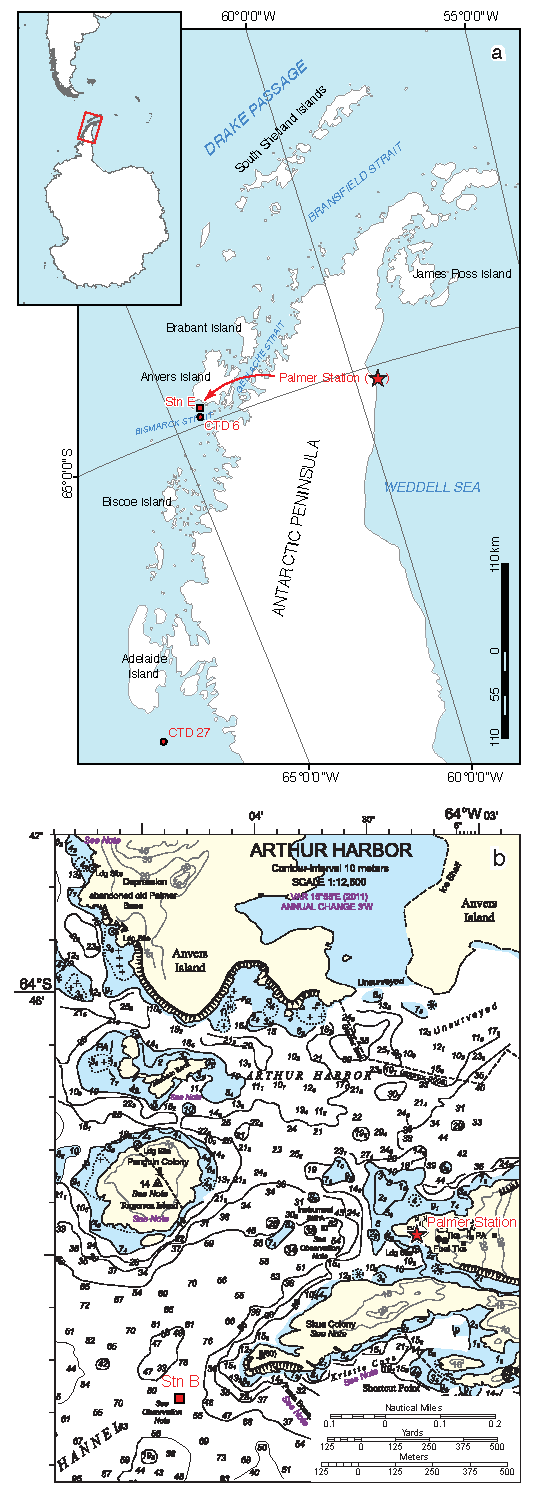
\includegraphics[width=.5\textwidth]{Fig_4-1.pdf}
\captionsetup{font={footnotesize}}
\caption[Map showing locations of sampling stations]{(a) Map of the West Antarctic Peninsula, showing locations of sampling stations referenced in the text (Palmer Long Term Ecological Research study stations B and E, \includegraphics[height=\fontcharht\font`\B]{images/Fig_4-Inline1.pdf}; CTD casts 6 and 27 during cruse LMG 14-01, \includegraphics[height=\fontcharht\font`\B]{images/Fig_4-Inline2.pdf}) and of Palmer Station (\includegraphics[height=\fontcharht\font`\B]{images/Fig_4-Inline3.pdf}). Inset shows extent of map view in relation to Antarctica and South America. (b) Detail from inset of U.S. National Geospatial Intelligence Agency (NGA) nautical chart 29123 (INT 9105), showing bathymetry and major marine features in immediate vicinity of Palmer Station.}
\label{fig:c4n1}
\end{SCfigure}Whereas the borosilicate glass attenuated a significant fraction of incoming radiation at wavelengths \textless{} 315 nm, the quartz transmitted nearly all incoming radiation in the UVB band (290-315 nm); we thus refer hereafter to the two treatments as ``-- UVB'' and ``+ UVB,'' respectively (\autoref{fig:c4n2}). To simulate surface-layer conditions in the adjacent coastal ocean, incubations were conducted in a large, outdoor, green-bottomed aquarium at a water depth of 0.6 m. The aquarium was left open to the sky for the duration of each experiment. The station's seawater intake system was used to circulate fresh seawater through the aquarium at a rate sufficient to gently agitate the incubation vessels; the rate of circulation also served to maintain the water at a constant temperature. Samples representing various light and microbial community treatments (described below) were sacrificed in triplicate at time points throughout the day while incoming solar radiation was measured \emph{in situ}. Total exposure times in the experiments ranged from 8.2 to 12.4 hours.

\subsubsection{Preparation of Phosphatidylcholine Liposomes}

For the experiments, artificial lipid membranes were prepared from liposomes of various species of phosphatidylcholine (PC; \autoref{fig:aen1}), a membrane lipid common to nearly all phyla, including marine microbial eukaryotes and prokaryotes. The use of liposomes prepared from molecular species of the investigator's choosing allows him or her to constrain the initial composition, fate, and potential products of lipid oxidation in experiments where a high degree of control and specificity is desired (Reis and Spickett, 2012). As a consequence, liposomes are frequently used as structural analogs for membrane lipids (Wagner et al., 1994) in studies of lipid function and oxidation in both plant (e.g., Zhou et al., 2009) and human (e.g., Thomas et al., 2010) cells; more recently, a liposome model was also used to investigate the antioxidant capacity of pigments produced by a marine bacterium (Correa-Llant\'{e}n et al., 2012). Experiments with liposomes can be particularly useful in photochemical studies when distinguishing among the many pathways through which lipids can be oxidized (Stratton and Liebler, 1997).

For this study, an Avanti Mini-Extruder and seven species of synthetic phosphatidylcholine containing fatty acid moieties of varying unsaturation and chain length (full list, \autoref{table:aen1}; molecular structures, \autoref{fig:aen1}) were obtained from Avanti Polar Lipids, Inc. (Alabaster, AL, USA). To improve yield during the extruding process, liposomes were prepared from lipid films rather than from the simple dry lipid mixture recommended by the manufacturer. Detailed protocols for preparation of both films and liposomes are available online; a link is provided at the end of the manuscript. To prepare the films, known quantities of each lipid dissolved in chloroform (approx. 200 $\mu$L) were dispensed into 20 mL precombusted, round-bottomed, screw-top glass vials using a solvent-washed glass syringe. The chloroform was then evaporated under a constant stream of nitrogen gas while the vial was revolved continuously by hand around its major axis. By gradual evaporation of the chloroform in this manner, the lipid was deposited as a thin film along the inside wall of each vial. Residual chloroform was removed via vacuum centrifugation (30 minutes), the vials flushed with argon, and screw-top threads sealed with Teflon (PTFE) film. The vials were then capped and stored until needed (in all instances, \textless{} 2 months) at --20$^{\circ}$C. The final quantity of lipid in each tube ranged from 500-2000 $\mu$g, depending on the species.

Fresh liposomes were extruded from these films 1-2 hours before the start of each experiment according to a modified version of the manufacturer protocol. Briefly, for each lipid to be evaluated, a film was retrieved from cold storage and hydrated with 500 $\mu$L of a buffer solution containing 260 mM NaCl and 50 mM Tris (both reagent grade, Fisher Scientific, USA). The tube was then incubated for one hour at 60$^{\circ}$C while subjected to gentle agitation. Using the Avanti Mini-Extruder, liposomes were then extruded from the lipid suspension by forcing the suspension multiple times through a single-use 0.2 $\mu$m polycarbonate membrane. The extruder was maintained at 60-70$^{\circ}$C by means of a hot plate. The protocol was repeated for as many lipids as required. Extruder components and syringes were rinsed between use and a new membrane was used for each lipid.

\subsubsection{Experimental Design and Treatments}

A different combination of liposomes was selected for each experiment (\autoref{table:aen1}) and extruded separately as described above. The different liposome suspensions were then combined into a single volume and gently mixed. The combined suspension was then dispensed into a precombusted glass beaker containing fresh natural seawater that had been passed three times through a 0.2 $\mu$m pore size Durapore hydrophilic membrane filter (Whatman); our intent was to exclude both phytoplankton and most of the heterotrophic bacteria, while retaining any dissolved organic matter present. The raw seawater was collected from the nearby harbor by means of a peristaltic pump; tubing was flushed with a 5 \% hydrochloric acid solution prior to sampling. In two of the five experiments (20 Nov. and 14 Dec. 2013), we employed an additional seawater matrix to evaluate whether the process of microbial degradation might enhance rates of lipid photooxidation. In these experiments, we divided the liposome suspension between equal volumes of the 0.2 $\mu$m-filtered seawater and seawater which had been passed three times through a GF/F glass fiber filter (nominal pore size 0.7 $\mu$m; Whatman). In the 0.7 $\mu$m-filtered fraction, we sought to exclude the majority of large-celled eukaryotic phytoplankton. We refer hereafter to the two treatments as ``-- het. bact.'' and ``+ het. bact.,'' respectively.\begin{SCfigure}[1][!b]
\centering
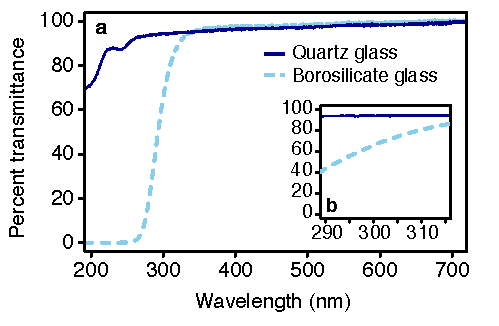
\includegraphics[width=.5\textwidth]{Fig_4-2.pdf}
\captionsetup{font={footnotesize}}
\caption[Transmission spectra of glass incubation vessels used in lipid photooxidation experiments]{(a) Transmission spectra of the glass incubation vessels used in lipid photooxidation experiments measured used a dual-path benchtop spectrophotometer. (b) Inset, showing transmissivities in the UVB spectral band (290-315 nm).}
\label{fig:c4n2}
\end{SCfigure}

After the liposome suspension was dispensed into one or both volume(s) of filtered seawater, a sufficient number of incubation vessels of the proper glass quality (quartz or borosilicate glass) were filled with the liposome-seawater solution(s) to permit evaluation in triplicate at several time points of all possible treatment combinations (-- and + UVB, and, in the case of the 20 Nov. and 14 Dec. experiments, -- and + het. bact.). To eliminate headspace, vials were filled to slightly overflowing. The mouths of the vials were then covered with PTFE film prior to stoppering (quartz vials) or securing with screw caps (borosilicate vials). Black electrical tape was used to further seal the outsides of the stoppers or screw caps to ensure vials did not inadvertently open during incubation. Sets of triplicate samples were also reserved in additional borosilicate glass vials for parallel incubation in the dark at \emph{in situ} temperature (hereafter, we refer to these as -- and + het. bact. ``dark controls'').

\subsubsection{Sampling and Extraction Protocol}

Samples were sacrificed and analyzed in triplicate at predesignated time points and the lipid content was recovered by liquid-liquid extraction. Each sample was transferred to a precombusted 200 mL glass separatory funnel and 30 $\mu$L of a synthetic IP-DAG (dinitrophenyl-phosphatidylethanolamine, or DNP-PE; Avanti) was immediately added at known concentration as an internal standard. 20 mL dichloromethane (HPLC grade; Sigma-Aldrich) was then added, followed by 50 $\mu$L of 45.4 mM butylated hydroxytoluene (BHT; 99.8 \%, Acros Organics) in HPLC-grade methanol (CHROMASOLV for HPLC; Sigma-Aldrich). This allowed us to achieve an effective concentration of the antioxidant of 0.0025\% (\emph{w/v}) in the organic phase (Yao et al., 2008). The funnel was then stoppered and mixed vigorously three times; phases were allowed to separate briefly between mixing. The organic phase (ca. 20 mL) was then collected into a precombusted glass vial and reduced in volume to approx. 1.5 mL using a nitrogen blowdown system. The final extract was transferred to a precombusted HPLC vial, topped with argon, and then stored at --80$^{\circ}$C until ready for analysis.

\subsubsection{Supplementary Assays Employed During Certain Experiments}

We employed additional assays during the 20 Nov. and 14 Dec. 2013 experiments to (1) validate our observations of lipid photooxidation with a standard measurement of lipid peroxidation and (2) interrogate bacterial metabolic activity in our + het. bact. treatments (i.e., those containing the 0.7 $\mu$m seawater filtrate). First, we adapted a commercial biomedical assay kit (ab118970 Lipid Peroxidation/MDA Assay Kit; Abcam Inc., Cambridge, UK) to detect the presence in our samples of malondialdehyde (MDA), a low-molecular-weight oxidation end-product of both enzymatically catalyzed (Armstrong and Browne, 1994) and abiotic (Janero, 1990) lipid peroxidation in a variety of organisms. The assay was carried out according to the manufacturer protocol for tissue/cell samples using 400 $\mu$L sample, 300 $\mu$L of the provided lysis buffer, and 6 $\mu$L BHT; a 510/535 nm excitation/emission filter pair was used for fluorometric detection and quantification of the MDA-thiobarbituric acid (TBA) adduct. In addition, activities of four bacterial exoenzymes (lipase, alkaline phosphatase, $\alpha$-D-glucosidase, aminopeptidase) were monitored throughout the experiments using a series of fluorogenic substrates (Hoppe, 1993) as described in Edwards et al. (2011). Briefly, pre-prepared 96-well plates containing the substrates were inoculated with aliquots of sample from each treatment; the plates were incubated in darkness at the same temperature as the water in the aquarium. The hydrolysis of these substrates and the attendant release of the free fluorophores 4-methylumbelliferone and 7-amino-4-methylcoumarin was monitored over time using a Tecan Infinite F200 Pro plate reader. External standard curves were used to convert fluorescence values to concentration units; enzyme hydrolysis rates were then calculated by linear regression from the observed changes in concentration. A detailed enzyme assay protocol and interactive MATLAB script for calculation of hydrolysis rates from raw fluorescence data are available online at \url{https://github.com/jamesrco/ExoenzymeHydroCalc}.

\subsection{Measurements of Incoming Irradiance}
\label{ssec:Measurements of Incoming Irradiance}

During the photooxidation experiments, an Ocean Optics Jaz spectrometer (ILX-511B detector; Ocean Optics Inc., Dunedin, FL, USA) was used to record incident irradiances \emph{in situ} at 0.3 nm bandwidth from 200-850 nm. Measurements were made in the aquarium at the same 0.6 m depth as the incubation vessels using an upward-facing plane irradiance cosine corrector and 5 or 10 m fiber optic cables that had been factory calibrated for absolute irradiance measurements from 210-850 nm. Irradiances were recorded at 1 min. intervals in units of $\mu$W cm\textsuperscript{-2}. The Jaz device was also used to record irradiances at 0.6 m for several extended periods from October-December 2013. Daily spectral integrals of total UVB and UVA irradiance (the time- and wavelength-integrated daily irradiance received between 290-315 nm and 315-400 nm, respectively, in a 24-hour period; reported in kJ m\textsuperscript{-2} d\textsuperscript{-1}) were calculated from these data for comparison with incident earth-surface irradiances recorded simultaneously at Palmer Station as part of the U.S. National Oceanic and Atmospheric Administration's (NOAA) Antarctic UV Monitoring Network (Bernhard et al., 2005; 2010; \autoref{fig:c4n3}).
\begin{figure}[!p]
\centering
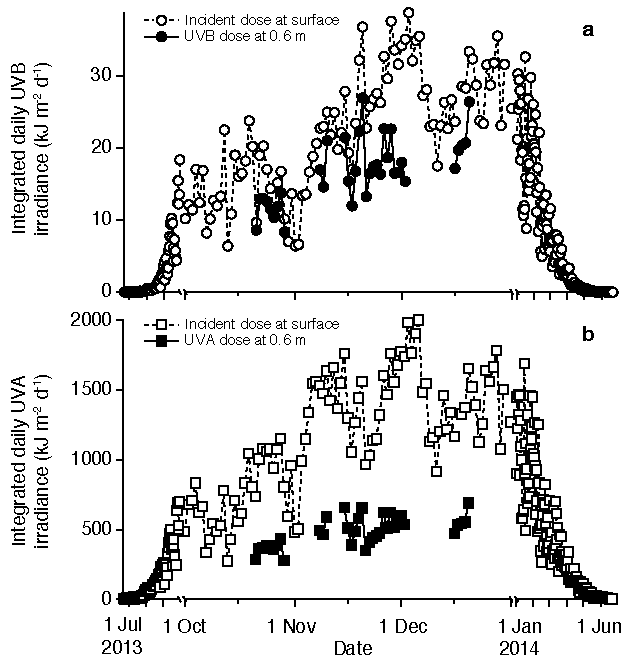
\includegraphics[width=.78\textwidth]{Fig_4-3.pdf}
\captionsetup{font={footnotesize}}
\caption[Daily doses of UVA and UVB radiation received at Palmer Station in 2013-2014]{Time- and wavelength-integrated daily doses of (a) UVB (290-315 nm) and (b) UVA (315-400 nm) radiation received at Palmer Station from 1 July 2013 to 30 June 2014. Open circles and squares: Incident doses measured at the earth surface from SUV-100 spectroradiometer data (courtesy U.S. National Oceanic and Atmospheric Administration (NOAA) Antarctic UV Monitoring Network, NOAA Global Monitoring Division, Boulder, CO, USA). Closed circles and squares (sections with expanded \emph{x}-axis): Downwelling UVB and UVA radiation received at 0.6 m below the ocean's surface, measured using a calibrated Ocean Optics Jaz spectrometer as described in the text. The largest daily dose of UVB radiation was received on 3 December 2013 even though the seasonal minimum in total column ozone (154.82 Dobson units) was recorded on 12 October 2013.}
\label{fig:c4n3}
\end{figure}

\subsubsection{Water Column Irradiance Profiles; Calculation of Downwelling Attenuation Coefficients (\emph{K\textsubscript{d}})}
\label{sssec:Water Column Irradiance Profiles; Calculation of Downwelling Attenuation Coefficients}

Finally, in 2013 and 2015, the Jaz was used to make several profiles of downwelling irradiance in the water column adjacent to Palmer Station in Arthur Harbor (e.g., \autoref{fig:c4n4}). All profiles were made at Station B, a sampling location occupied twice weekly during the austral summer as part the Palmer Long Term Ecological Research (PAL-LTER) study (\autoref{fig:c4n1}b). To achieve minimum boat shadow while making the profile measurements, the fiber optic cable and light sensor (cosine corrector) were streamed away from the small boat in a direction that was both to windward and toward the sun; the boat was then allowed to drift downwind from the measurement location to a suitable stand-off distance. Spectra were obtained at a range of depths from 0 to 8 m on days when few or no clouds were present. A series of concurrent surface irradiance measurements made with a LI-COR PAR sensor (model LI-193SA; LI-COR Biosciences, Lincoln, NE, USA) was used to correct the spectra made as part of these profiles for any changes in incident light intensity that occurred between measurements. The PAR sensor was mounted in a fixed location on the small boat such that it enjoyed a constant, unobstructed path to the sun. The corrected irradiances were used to calculate a series of wavelength-dependent downwelling attenuation coefficients, ${K_d}(\lambda )$, for wavelengths from 290-700 nm, according to:
\begin{equation} \label{eq:c4e1}
{I_z}(\lambda ) = {I_0}{(\lambda )^{ - {K_d}(\lambda )z}}
\end{equation}
where ${I_z}(\lambda )$ is the spectral irradiance at depth irradiance $z$ and ${I_0}(\lambda )$ is the spectral irradiance just below the sea surface. Values of ${K_d}(\lambda )$ are given in \autoref{table:aen2}. Where necessary for apparent quantum yield (AQY) calculations (\autoref{ssec:Calculation of Broadband Polychromatic Apparent Quantum Yields (AQY)}, below), we also converted downwelling irradiances to wavelength-specific photon fluxes (${E_p}(\lambda )$, in units of $\mu$mol photons m\textsuperscript{-2} s\textsuperscript{-1}) using the equation
\begin{equation} \label{eq:c4e2}
{E_p}(\lambda ) = I(\lambda ) \times \lambda  \times 0.836 \times {10^{ - 2}}
\end{equation}
where $\lambda$ is a given wavelength in nm, ${I}(\lambda )$ is the irradiance in W m\textsuperscript{-2}, and the additional numerical coefficients are used to effect necessary conversions via Planck's equation and Avogadro's number.
\begin{figure}[!t]
\centering
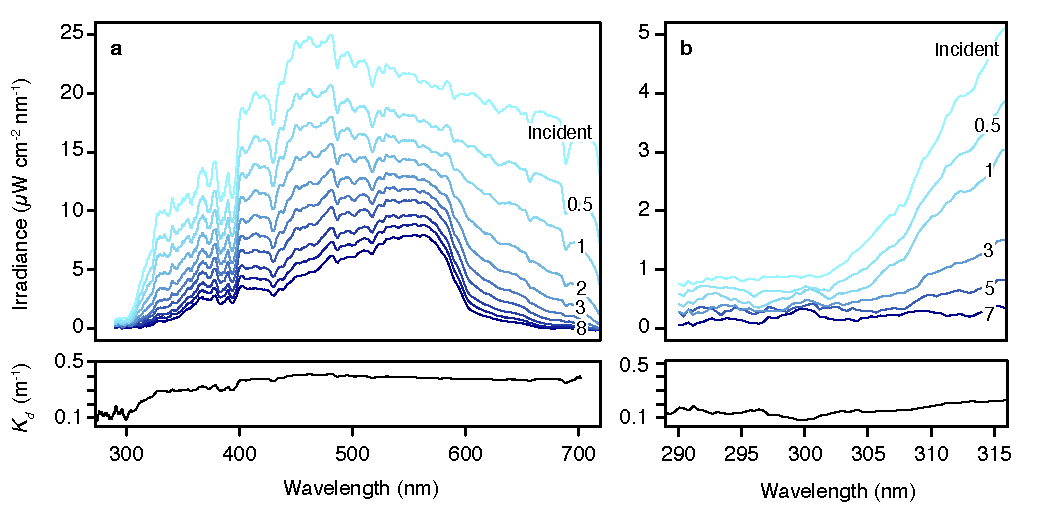
\includegraphics[width=1\textwidth]{Fig_4-4.pdf}
\captionsetup{font={footnotesize}}
\caption[Wavelength-specific measurements of downwelling irradiance in Arthur Harbor]{Wavelength-specific measurements of downwelling irradiance in Arthur Harbor (PAL-LTER Station B) on 15 December 2015. Labels refer to depths in meters below the sea surface. (a) UV-visible spectra (290-700 nm) at 10 depths. Data from 1-8 m are plotted at 1 m intervals. (b) Inset showing UVB-band (290-315 nm) irradiances at selected depths. Bottom panels show downwelling attenuation coefficients for each wavelength, ${K_d}(\lambda )$, which were calculated from the data according to \autoref{eq:c4e1} in the text. ${K_d}(\lambda )$ for wavelengths 280-700 nm are given in \autoref{table:aen2}.}
\label{fig:c4n4}
\end{figure}

\subsection{Benchtop Absorbance and Transmissivity Measurements}
\label{ssec:Benchtop Absorbance and Transmissivity Measurements}

Wavelength-specific absorbances of various PC lipid standards (dissolved in HPLC-grade methanol; \autoref{fig:c4n5}) and seawater samples from surface waters in Arthur Harbor (\autoref{fig:aen2}) were measured in the laboratory using a dual-path UV-visible spectrophotometer (Thermo Nicolet Evolution 300; ThermoFisher Scientific). 100 mm quartz cuvettes were used for all measurements. HPLC-grade methanol and 0.2 $\mu$m-filtered oligotrophic ocean seawater (collected from 50 m at the Bermuda-Atlantic Time Series site, 32$^{\circ}$ 10' N, 64$^{\circ}$ 30' W) were used as references for the two sample types, respectively. Absorbance spectra of the liposome standards (\autoref{fig:c4n5}a,b) were used to calculate wavelength-specific decadic molar extinction coefficients (${\varepsilon _i}(\lambda )$, in units of M\textsuperscript{-1} cm\textsuperscript{-1}; \autoref{fig:c4n5}c) using the equation
\begin{equation} \label{eq:c4e3}
{\varepsilon _i}(\lambda ) = {A_i}(\lambda ) \times {C_i} \times \ell 
\end{equation}
where ${A_i}(\lambda )$ is the absorption at wavelength $\lambda$, $\ell$ is the pathlength (10 cm), and ${C_i}$ is the concentration of the relevant analyte (liposome standard) in units of mol L\textsuperscript{-1}. Raw absorbances of the seawater samples (${A_{SW}}(\lambda )$) were used to calculate wavelength-specific seawater absorbance coefficients (${a_{SW}}(\lambda )$, in units of m\textsuperscript{-1}; \autoref{fig:aen2}) according to:
\begin{equation} \label{eq:c4e4}
{a_{SW}}(\lambda ) = {A_{SW}}(\lambda ) \times 2.303/\ell 
\end{equation}
Transmission spectra of the glass incubation vessels (\autoref{ssec:UV Photooxidation Experiments}, above; \autoref{fig:c4n2}) were recorded using the same instrument on which the liposome and seawater absorbance spectra were acquired.

\subsection{Laboratory Determination of H\textsubscript{2}O\textsubscript{2} and O\textsubscript{2}\textsuperscript{-} Photoproduction and Decay}
\label{ssec:Laboratory Determination of ROS Photoproduction and Decay}

In a series of subsequent experiments in the laboratory in Woods Hole, net hydrogen peroxide (H\textsubscript{2}O\textsubscript{2}) and superoxide (O\textsubscript{2}\textsuperscript{-}) photoproduction rates were estimated in surface seawater samples from Arthur Harbor. H\textsubscript{2}O\textsubscript{2} concentrations were determined using the colorimetric Ampliflu Red method described in Zhang et al. (2016a). O\textsubscript{2}\textsuperscript{-} concentrations were measured with a continuous-flow FeLume Mini system (Waterville Analytical, Waterville, ME, USA) configured as described in Zhang et al. (2016b). In the experiments, previously frozen, 0.7 $\mu$m-filtered seawater samples were excited at a series of wavelengths using the spectrophotometer described in \autoref{ssec:Benchtop Absorbance and Transmissivity Measurements}; concentrations of H\textsubscript{2}O\textsubscript{2}) and superoxide (O\textsubscript{2}\textsuperscript{-} were then measured using the methods described above. To evaluate photoproduction rates of H\textsubscript{2}O\textsubscript{2}, we excited samples at 280, 310, and 360 nm based on the findings of Kieber et al. (2014); for O\textsubscript{2}\textsuperscript{-}, we evaluated a broader wavelength range (50-nm-wavelength increments from 300-500 nm; Powers and Miller, 2015). Sample water was passed through beam of the spectrophotometer using a peristaltic pump and 10 mm pathlength flow-cell while the xenon lamp was operated in continuous (i.e., not flash) mode at the desired wavelength. Opaque (black) tubing was used, and all other components were triple-shielded using aluminum foil. Downstream of the spectrophotometer beam, the sample was either pumped directly into the FeLume (for O\textsubscript{2}\textsuperscript{-}) or expediently assayed for H\textsubscript{2}O\textsubscript{2}. The intensity of the xenon lamp output in the UVB range (determined using the Jaz spectrometer described in \autoref{sssec:Water Column Irradiance Profiles; Calculation of Downwelling Attenuation Coefficients}) was roughly equivalent to the downwelling UVB irradiances we observed at 1 m in Arthur Harbor (the lamp output at 290 nm was 0.43 $\mu$W cm\textsuperscript{-2}, compared with 0.42 $\mu$W cm\textsuperscript{-2} at 1 m in the profile presented in \autoref{fig:c4n4}). At wavelengths \textgreater{} 315 nm, the spectrophotometer output was significantly less intense than what was observed in the water column. In a final set of experiments, the ability of Arthur Harbor seawater to quench (i.e., degrade) H\textsubscript{2}O\textsubscript{2} and O\textsubscript{2}\textsuperscript{-} was estimated by measuring concentrations of the two ROS after spiking the samples with progressively larger concentrations of potassium superoxide (KO\textsubscript{2}).
\begin{SCfigure}[1][!t]
\centering
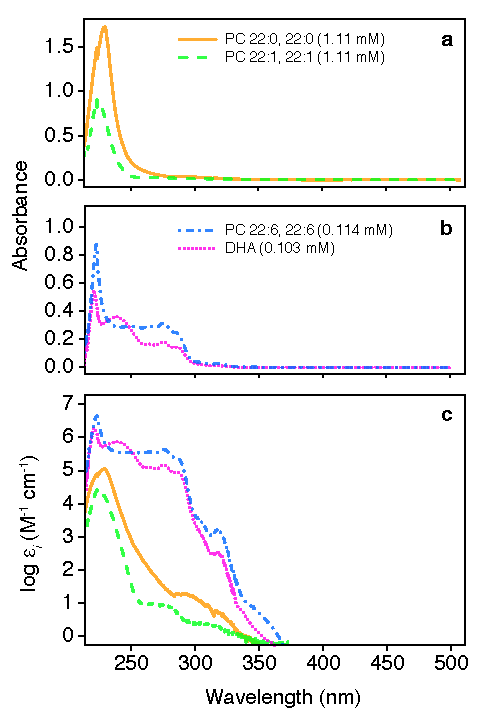
\includegraphics[width=.56\textwidth]{Fig_4-5.pdf}
\captionsetup{font={footnotesize}}
\caption[Wavelength-specific absorbances and decadic molar extinction coefficients of phosphatidylcholine and DHA]{Effect of acyl unsaturation on photochemical potential in the membrane lipid phosphatidylcholine (PC) and constituent fatty acid docosahexaenoic acid (DHA). (a) Wavelength-specific absorbances of equimolar (1.11 mM) concentrations of PC 22:0, 22:0 and PC 22:1, 22:1 (\emph{cis}-$\Delta$\textsuperscript{13}) dissolved in methanol. (b) Wavelength-specific absorbances of PC 22:6, 22:6 (\emph{all-cis}-$\Delta$\textsuperscript{4},$\Delta$\textsuperscript{7},$\Delta$\textsuperscript{10},$\Delta$\textsuperscript{13},$\Delta$\textsuperscript{16},$\Delta$\textsuperscript{19}) and DHA at concentrations in methanol of 0.114 and 0.103 mM, respectively. (c) Decadic molar extinction coefficients, ${\varepsilon _i}(\lambda )$, for the four species, calculated according to \autoref{eq:c4e3} in the text. Note logarithmic scale on the \emph{y}-axis.}
\label{fig:c4n5}
\end{SCfigure}

\subsection{Water Column Sample Collection}

In addition to the photooxidation experiments, several water samples were collected for lipid analysis in 2013-2014 from waters of the adjacent harbor (at LTER Station B; \autoref{fig:c4n1}b) and on an oceanographic research cruise off the West Antarctic Peninsula (PAL-LTER cruise LMG1401 aboard the \emph{R/V Laurence M. Gould}). Persistent sea ice in the immediate vicinity of Palmer Station prevented regular collection of samples there until mid-December 2013; samples from the \emph{Gould} cruise were collected in January 2014 at distances of 50-300 km from shore. Samples for analysis of particulate (i.e., cell-bound) lipids were retrieved from depth using standard oceanographic sampling equipment and then collected by vacuum filtration onto 0.2 $\mu$m pore size Durapore membrane filters; these were frozen immediately at --80$^{\circ}$C. For analysis of total lipids, we used the liquid-liquid method described above to extract 2000 mL of seawater into 200 mL dichloromethane in a 2 L separatory funnel; 120 $\mu$L of DNP-PE and 100 $\mu$L BHT were added as internal standard and preservative antioxidant, respectively. Extraction of particulate samples was performed using a modified Bligh and Dyer (Bligh and Dyer, 1959) method described in Popendorf et al. (2013). Extracts were processed and then stored at --80$^{\circ}$C as described above.

\subsection{High-Resolution HPLC-ESI-MS Analysis}

Lipid extracts were analyzed by HPLC-ESI-MS with data dependent-MS\textsuperscript{2} acquisition on a high-resolution, accurate mass Thermo Q Exactive Hybrid Quadrupole-Orbitrap mass spectrometer (ThermoFisher Scientific, Waltham, MA, USA) coupled to an Agilent 1200 HPLC system (Agilent, Santa Clara, CA, USA) comprising a temperature-controlled autosampler (4$^{\circ}$C), binary pump, and diode array detector. Chromatographic conditions were modified from Hummel et al. (2011). High-resolution mass data were acquired in both positive and negative ionization modes; following the full spectrum scan in each mode, the five ions of highest intensity were selected using the quadrupole for MS\textsuperscript{2} fragmentation. Full details, including chromatographic conditions, electrospray ionization source settings, MS acquisition settings, and mass spectrometer calibration procedures, are described in the Supporting Information (\autoref{ssec:Mass Spectrometer Acquisition Settings}); the method allowed us to achieve an effective mass accuracy of \textless{} 0.2 ppm, as reported in Collins et al. (2016). All chemicals used in sample extraction and chromatography were LC/MS grade or higher. Where used, water was obtained from a Milli-Q system without further treatment (EMD Millipore, Billerica, MA, USA).

\subsubsection{Identification and Quantification of Lipids \& Oxidized Lipids}
\label{sssec:Chap 4 - Identification and Quantification of Lipids and Oxidized Lipids}

HPLC-ESI-MS data were processed in R (R Core Team, 2016) using msConvert (Kessner et al., 2008), xcms (Benton et al., 2010; C. A. Smith et al., 2006; Tautenhahn et al., 2008), and CAMERA (Kuhl et al., 2012) according to the steps described in Collins et al. (2016). The R package IPO (Libiseller et al., 2015) was used to optimize some xcms settings. The LOBSTAHS lipidomics discovery software (Collins et al., 2016) was used to extract and putatively identify MS features in both the experimental and environmental data. In data from the liposome experiments, we identified the added PC species, any possible degradation products, and the internal standard, DNP-PE. For intact PC species, DNP-PE, and constituent fatty acids, we confirmed each LOBSTAHS identification using two additional means: (1) via comparison of data-dependent MS\textsuperscript{2} spectra with those from authentic standards or published reference spectra and (2) by requiring the presence of the same compound identity in data acquired in the opposite HPLC-ESI-MS ionization mode. We confirmed the basic identities of the LPC and ox-PC species based on the presence of four or more diagnostic PC headgroup fragments in the relevant MS\textsuperscript{2} spectrum. In the more complex environmental samples and in single-species culture data, we confirmed all LOBSTAHS identities at the lipid class level (e.g., PC versus PE, or MGDG versus TAG) using a new, experimental LOBSTAHS feature which automatically detects diagnostic product ion fragments and constant neutral losses (as given in Popendorf et al., 2013) in the available data-dependent MS\textsuperscript{2} spectra for each sample. In addition, we required the presence of the same LOBSTAHS compound identity in data acquired in the opposite HPLC-ESI-MS ionization mode, as described above for the experimental data.

After identification, quantification of analytes was performed using a series of standard curves. For quantification of IP-DAG, authentic standards were obtained either from natural extracts or from the same source (Avanti Polar Lipids) as the lipids used in the liposomes (Popendorf et al., 2013; Van Mooy and Fredricks, 2010). For quantification of docosahexaenoic acid (DHA), an authentic standard was obtained from Nu-Chek Prep Inc. (Elysian, MN, USA). For LPC and ox-PC species, we applied the standard curve for the corresponding intact, unoxidized molecule; authentic standards are commercially available for only a small fraction of the many possible intact ox-PC species and their isomers. The concentration of each analyte was then normalized to the concentration in the same sample of the internal standard.

\subsection{Calculation of Broadband Polychromatic Apparent Quantum Yields (AQY)}
\label{ssec:Calculation of Broadband Polychromatic Apparent Quantum Yields (AQY)}

We combined the removal rates (where observed) of PC species determined in the liposome experiments, \emph{in situ} photon flux measurements, and other parameters described above to calculate a series of broadband (as in, e.g., Fichot and Benner, 2014) polychromatic apparent quantum yields, ${\Phi _{{\lambda _1}:{\lambda _2}}}$, where
\begin{singlespace}
\begin{equation} \label{eq:c4e5}
{\Phi _{{\lambda _1}:{\lambda _2}}} = \frac{{{\text{moles of a given lipid }}i{\text{ transformed}}}}{\begin{gathered}
  {\text{no. of moles of photons between wavelenths }} \\ 
  {\lambda _1}{\text{ and }}{\lambda _{\text{2}}}{\text{ absorbed due to the presence of }}i \\ 
\end{gathered} }
\end{equation}
\end{singlespace} 
\hfill\break
We calculated these yields according to the equation:
\begin{equation} \label{eq:c4e6}
{\Phi _{{\lambda _1}:{\lambda _2}}} = \frac{{\frac{{ - d[i]}}{{dt}}}}{{[i]\int\limits_{{\lambda _1}}^{{\lambda _2}} {{K_s}(\lambda )d\lambda } }}
\end{equation}
where ${\Phi _{{\lambda _1}:{\lambda _2}}}$ is the broadband polychromatic AQY in units of mol (mol photons)\textsuperscript{-1}, $ - d[i]/dt$ is the change in concentration of lipid \emph{i} in a given experimental treatment, $[i]$ is the concentration of \emph{i} measured in the experiment at \emph{t} = 0 (i.e., prior to photon exposure), and ${K_s}(\lambda )$ are the time-integrated specific absorbances of \emph{i} calculated at wavelengths from ${\lambda _1}$ to ${\lambda _2}$. Our experimental design allowed us to calculate AQY for three wavelength ranges: ${\Phi _{290:315}}$ (or ${\Phi _{UVB}}$, for radiation received in the UVB band), ${\Phi _{315:395.5}}$ (${\Phi _{UVA}}$, for radiation received in the UVA band), and ${\Phi _{290:395.5}}$ (or ${\Phi _{UVR}}$, a yield based on the total received UV radiation).

We used a different definition of $ - d[i]/dt$ for calculation of the three AQY; these hewed closely to the observed transmittance spectra of the various treatment vessels (\autoref{fig:c4n2}). In all three cases, we assumed the change in concentration of PC 22:6, 22:6 in the dark control treatment (-39 $\pm$ 23 pmol mL\textsuperscript{-1} hr\textsuperscript{-1}; \autoref{table:c4n1} and \autoref{fig:c4n6}a) represented the baseline rate of autooxidation, a process common to all lipids containing unsaturated acyl moieties but often more significant in those containing highly polyunsaturated fatty acids (Girotti, 1998). For ${\Phi _{UVR}}$, we therefore defined $ - d[i]/dt$ as the change in concentration observed in the +UVB (quartz glass) treatment relative to the change in the dark control. For calculation of ${\Phi _{UVA}}$, we applied the concentration change observed in the --UVB (borosilicate glass) treatment, again correcting for the dark oxidation rate. Finally, for calculation of ${\Phi _{UVB}}$, the efficiency of photooxidation attributable only to UVB radiation, we defined $ - d[i]/dt$ as the difference between the changes in concentration observed in the -- UVB and + UVB treatments. ${K_s}(\lambda )$ were calculated after Pereira et al. (2007) according to the equation
\begin{equation} \label{eq:c4e7}
{K_s}(\lambda ) = \frac{{E_{p,\Sigma }^o(\lambda )T(\lambda ){\varepsilon _i}(\lambda )(1 - {{10}^{ - {a_{SW}}(\lambda ){z_{eff}}}})}}{{{a_{SW}}(\lambda ){z_{eff}}}}
\end{equation}	
where $E_{p,\Sigma }^o(\lambda )$ is the total number of photons of wavelength $\lambda$ received per unit area over the course of the experiment, i.e.,
\begin{equation} \label{eq:c4e8}
E_{p,\Sigma }^o = \int\limits_{t = 0}^{t = f} {E_p^o(\lambda )dt} 
\end{equation}	
$T(\lambda )$ is the transmissivity (as a fraction) of the incubation vessel wall material at wavelength $\lambda$, ${\varepsilon _i}(\lambda )$ is the experimentally-determined decadic molar extinction coefficient at wavelength $\lambda$ (from \autoref{eq:c4e3}), and ${a_{SW}}(\lambda )$ and $(1 - {10^{ - {a_{SW}}(\lambda ){z_{eff}}}})$ are the wavelength-specific absorbance coefficient (m\textsuperscript{-1}) and fraction of radiation absorbed by the seawater in the incubation vessel along the effective path length ${z_{eff}}$, respectively. For ${z_{eff}}$, we applied one-half the inner diameter of the incubation vessels ($0.5\times2$ cm = 1 cm) since the vessels were left to rest almost exclusively on their sides during the experiments and were exposed to sunlight from above.

\subsubsection{Determination of Uncertainties in AQY Estimates}
\label{sssec:Determination of Uncertainties in AQY Estimates}

We used a series of Monte Carlo-style computational simulations to determine uncertainties in our final estimates of AQY. The method used was similar to that described in Collins et al. (2015). First, where possible, we determined uncertainties for all individual parameters in \autoref{eq:c4e6}, \autoref{eq:c4e7}, and \autoref{eq:c4e8} from experimental replication or, in the case of data obtained from single samples using the benchtop spectrophotometer, repeated analytical measurements. We then conducted a series of 10,000 simulations in which a new value for each parameter was chosen at random from a normal distribution constructed from the parameter's mean value and analytical or observational uncertainty as its standard deviation. In each simulation, the randomly chosen values from these normal distributions were used to obtain a different estimate of the AQY from \autoref{eq:c4e6}, \autoref{eq:c4e7}, and \autoref{eq:c4e8}. The final uncertainty in each AQY estimate was determined from the standard deviation of the set of estimates generated during the simulation. The R code we used to conduct the simulation is available online; a link is provided in the Supporting Information. Although we constructed normal distributions for each parameter in the simulations, we could not be absolutely certain the underlying populations were normally distributed because of the small sample sizes.

\subsection{Lipid Photooxidation Rate Estimates}

Finally, we estimated rates of lipid photooxidation in natural waters of the West Antarctic Peninsula by combining our estimates of AQY with direct observations of subsurface irradiance and measured concentrations of specific lipids. Rates were estimated for two fractions of the lipids we measured in WAP waters: IP-DAG containing (1) polyunsaturated (i.e., $\geq$ 3 double bonds) and (2) highly polyunsaturated (i.e., $\geq$ 5 double bonds) fatty acids at both positions (\emph{sn-­}1 and \emph{sn-}2) on the IP-DAG glycerol backbone. Photooxidation rates ($ - d[i]/dt$; units of pmol lipid or pmol C d\textsuperscript{-1}) were calculated according to \autoref{eq:c4e6}, where ${\Phi _{{\lambda _1}:{\lambda _2}}}$ was the broadband polychromatic AQY for the UVB spectrum (${\Phi _{290:315}}$, or ${\Phi _{UVB}}$) and $[i]$ was the measured concentration (in pmol L\textsuperscript{-1}) of lipids in the respective fraction. We calculated the necessary ${K_s}(\lambda )$ according to
\begin{equation} \label{eq:c4e9}
{K_s}(\lambda ) = \frac{{E_{p,\Sigma }^o(\lambda ){\varepsilon _i}(\lambda )(1 - {{10}^{ - {K_d}(\lambda ){z_{surf}}}})}}{{{K_d}(\lambda ){z_{surf}}}}
\end{equation}	
where $E_{p,\Sigma }^o(\lambda )$ was a daily flux ($\mu$mol photons m\textsuperscript{-2} d\textsuperscript{-1}) calculated from the time-series of \emph{in situ} irradiance measurements described in \autoref{ssec:Measurements of Incoming Irradiance}, ${\varepsilon _i}(\lambda )$ was the experimentally-determined decadic molar extinction coefficient for the unsaturated compound, PC 22:6, 22:6, at wavelength $\lambda$, ${K_d}(\lambda )$ was the appropriate downwelling attenuation coefficient for Arthur Harbor calculated in \autoref{eq:c4e1}, and ${z_{surf}}$ was the depth of the well-mixed surface layer (5 m). We applied the measured ${\varepsilon _i}(\lambda )$ for PC 22:6, 22:6 to all lipids containing multiple polyunsaturated fatty acids based on our observations of the effect of polyunsaturation on specific absorbance in IP-DAG (\autoref{fig:c4n5}); in addition, it would have been highly impractical within the scope of the present work to measure specific ${\varepsilon _i}(\lambda )$ for the hundreds of different IP-DAG we observed in the natural samples.

\section{Results}
\subsection{Irradiance Observations; UV Penetration Through Shallow Mixed Layer}
\label{ssec:Irradiance Observations; UV Penetration Through Shallow Mixed Layer}

Comparison of daily UVB-band integrals calculated from our \emph{in situ} data (\autoref{fig:c4n3}a, filled circles) with integrals calculated from the incident NOAA data (\autoref{fig:c4n3}a, open circles) indicated that 70 $\pm$ 11 \% of the UVB radiation received at the earth's surface reached the 0.6 m depth at which we conducted our experiments (mean $\pm$ SD of 35 daily observations). A parallel calculation using UVA-band integrals indicated that 37 $\pm$ 3 \% of incident UVA radiation was received at 0.6 m (\autoref{fig:c4n3}b). While these findings are inconsistent with evidence from the majority of marine systems that UVB radiation is attenuated more rapidly with depth than lower-energy UVA radiation (Tedetti and Semp\'{e}r\'{e}, 2006), Figueroa (2002) found that ${K_d}(\lambda )$ for UVA wavelengths exceeded those for UVB wavelengths at two coastal sites very near Palmer Station.

Our profile measurements of downwelling irradiance (\autoref{fig:c4n4}) indicated that much of the UVB radiation at wavelengths \textless{} 300 nm was quickly attenuated in the water column; however, some UVB and a significant proportion of UVA radiation penetrated to depths of \textgreater{} 5 m. Our data confirm the findings of Moreau et al. (2015), who found that ecologically relevant doses of UVB radiation (i.e., doses $\geq$ 1 \% of surface intensity, the same standard used for determination of euphotic zone depth) were received at depths as great as 12 m in some West Antarctic Peninsula waters. Perhaps most importantly, this optical penetration was sufficient to expose nearly all of the shallow early-season mixed layer (\autoref{fig:aen3}) to robust doses of UV radiation throughout the study period. Typical mid-season mixed layer depths in Arthur Harbor range from 10-20 m (Tortell et al., 2014). Yet shallow MLDs of just 5-10 m, such as those we observed in 2013, are not unusual in the early spring following the breakup and retreat of the sea ice, which can create a highly stratified surface layer that traps both nutrients and ice-attached algae at the ocean's surface as they are released from the melting ice (Perrette et al., 2011; W. O. Smith and Nelson, 1985; 1986). A comparable surface lens may also be present throughout the season in coastal waters that receive significant inputs of glacial meltwater and in offshore waters at the persistent marginal ice zone (Carvalho et al., 2016; Huang et al., 2012). CTD profiles from PAL-LTER Station B (\autoref{fig:aen3}) indicate that the 2013-2014 season was not atypical in this regard, although the ice retreat occurred much later than usual.
\begin{SCfigure}[1][!t]
\centering
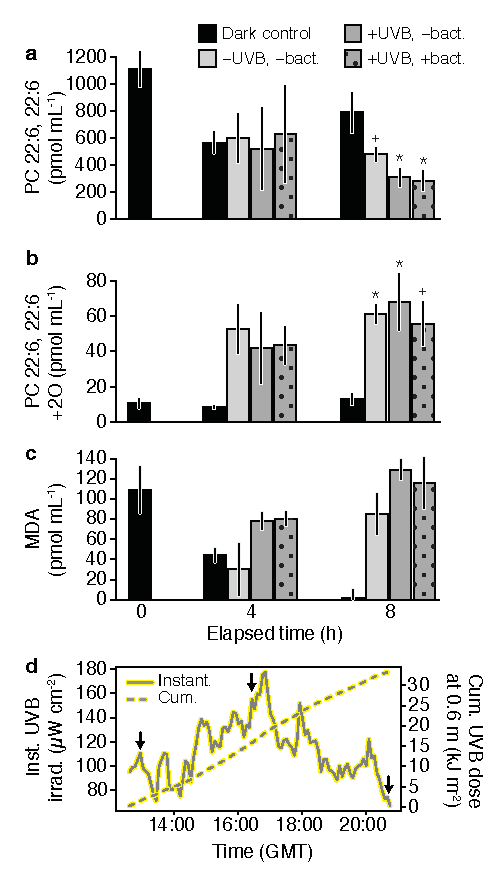
\includegraphics[width=.6\textwidth]{Fig_4-6.pdf}
\captionsetup{font={footnotesize}}
\caption[Results from a lipid photooxidation experiment conducted with phosphatidylcholine (PC) liposomes]{Results from a lipid photooxidation experiment conducted with phosphatidylcholine (PC) liposomes at Palmer Station on 14 December 2013. Concentrations after 4 and 8 h of (a) PC 22:6, 22:6, (b) an intact oxidation product (PC 22:6, 22:6 +2O; identified at chromatographic retention time 10.4 min.), and (c) malondialdehyde, a commonly-used indicator of lipid peroxidation activity. Error bars: $\pm$ SE of mean (initial concentrations, \emph{N} = 4 replicates; all other treatments and time points, \emph{N} = 3). Symbols in (a) and (b) indicate statistical significance of mean from initial concentration (value at \emph{t} = 0) according to Tukey's ``Honest Significant Difference'' method with $\alpha$ = 0.05: \emph{p} $\leq$ 0.05 (+), \emph{p} $\leq$ 0.01 (*). (d) Instantaneous (solid line) and cumulative (dashed line) UVB-band downwelling irradiance measured at the incubation depth (0.6 m). Arrows in (d) correspond to the times in (a)-(c) at which samples were sacrificed.}
\label{fig:c4n6}
\end{SCfigure}

\subsection{Rates of Photooxidation in Phosphatidylcholine Liposome Experiments}

Rates of photooxidation under exposure to natural sunlight were statistically significant in only one of the seven PC species we considered in our liposome experiments: PC 22:6, 22:6 (\emph{all-cis}-$\Delta$\textsuperscript{4},$\Delta$\textsuperscript{7},$\Delta$\textsuperscript{10},$\Delta$\textsuperscript{13},$\Delta$\textsuperscript{16},$\Delta$\textsuperscript{19}) (\autoref{fig:c4n6}a, showing results from experiment on 14 December 2013). Photooxidation rates of 80 $\pm$ 16, 98 $\pm$ 17 and 100 $\pm$ 17 pmol mL\textsuperscript{-1} hr\textsuperscript{-1} of the molecule were observed in the --UVB --het. bact., +UVB --het bact., and +UVB +het. bact. treatments, respectively (mean $\pm$ SE; \autoref{table:c4n1}). While we observed no statistical difference between these three rates, the rates in all three treatments were significantly different than the rate observed in the control treatment, 39 $\pm$ 23 pmol mL\textsuperscript{-1} hr\textsuperscript{-1} (\emph{p} $\leq$ 0.05; \autoref{table:c4n1}). In a second experiment for which results were not statistically significant (\autoref{table:aen1}), we recorded a photooxidation rate for liposomes of the same molecule of 57 $\pm$ 45 pmol mL\textsuperscript{-1} hr\textsuperscript{-1} in the +UVB --het bact. treatment. The consistently negative results we observed in the six other molecular species were confirmed in each case in at least two independent experiments (\autoref{table:aen1}). Differences in photooxidation rates were assessed within each experiment using Tukey's ``Honest Significant Difference'' method ($\alpha$ = 0.05), which takes into account the total variance in an experimental dataset when making multiple, simultaneous pairwise comparisons among treatments and timepoints (Yandell, 1997). Based on concentrations of PC 22:6, 22:6 observed in \emph{t} = 0 samples from the experiment for which we present results in \autoref{fig:c4n6} and \autoref{table:c4n1}, we recovered 80.5 \% of our starting lipid film as liposomes (\emph{t} = 0 concentration, 1108 $\pm$ 125 pmol mL\textsuperscript{-1}; calculated concentration based on known mass of lipid film, 1376.1 pmol mL\textsuperscript{-1}).

\subsection{Role and Activity of Heterotrophic Bacteria}
\subsubsection{No Evidence for Direct Bacterial Metabolism of Unoxidized Lipids}
\begin{figure}[!p]
\centering
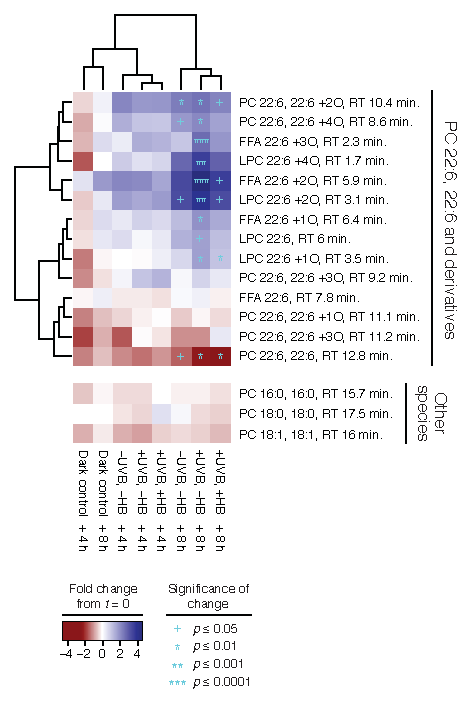
\includegraphics[width=.8\textwidth]{Fig_4-7.pdf}
\end{figure}

We observed a small marginal enhancement in the apparent degradation rate of PC 22:6, 22:6 liposomes in the +UVB treatment when heterotrophic bacteria were present, but this increase was not statistically significant (\autoref{fig:c4n6}a; \autoref{table:c4n1}). We had initially hypothesized that (1) bacterial metabolism of intact lipids present in the liposomes might enhance apparent overall degradation rates as the organisms responded to the addition of a new potential food source and that (2) bacterial metabolism might be further stimulated by photodegradation of the added lipids into smaller, less complex metabolites that could be more readily assimilated as substrates for growth. Several studies (e.g., Karl and Resing, 1993; D. J. Kieber et al., 1989) have suggested that photochemical degradation of dissolved organic matter in the surface ocean can stimulate the microbial loop by breaking down large, biologically refractory molecules into smaller, more bioavailable components. Despite some evidence that high doses of UVR can severely inhibit rates of metabolism in marine heterotrophic bacteria (Santos et al., 2011), two thorough reviews of the relevant literature (Jeffrey et al., 2000; Moreau et al., 2016) suggest that no single generalization can be made about the effect of ultraviolet radiation on marine bacterial communities: The \begin{figure} [!t]
\captionsetup{font={footnotesize}}
\captionof{figure}[Changes in the concentration of PC 22:6, 22:6 and various molecular derivatives during the liposome photooxidation experiment presented in \autoref{fig:c4n6}]{(preceding page) Changes in the concentration of PC 22:6, 22:6 and various molecular derivatives during the liposome photooxidation experiment presented in \autoref{fig:c4n6}. For a given treatment and time point on the \emph{x}-axis, cell color shows the fold change in concentration of each molecule on the \emph{y}-axis relative to the concentration observed at the initial experimental timepoint. Fold-change calculations are based on mean concentrations measured at each treatment and time point in at least 3 replicates. The order of both rows (analytes) and columns (treatment-time point combinations) reflects application of an unsupervised clustering algorithm. The dendrogram shows similarity (by Euclidean distance) among analytes and treatments/time points. Symbols in cyan indicate the statistical significance of the difference of each mean concentration relative to the mean concentration at the initial time point according to Tukey's ``Honest Significant Difference'' method with $\alpha$ = 0.05: \emph{p} $\leq$ 0.05 (+), \emph{p} $\leq$ 0.01 (*), \emph{p} $\leq$ 0.001 (**), \emph{p} $\leq$ 0.0001 (***). The lower subplot shows changes in concentration observed in the other PC species evaluated in the same experiment; no significant changes were observed in any of the species containing fully saturated or monounsaturated fatty acids. The heatmap was generated in R (R Core Team, 2016) using the gplots (Warnes et al., 2016) package.}
\label{fig:c4n7}
\end{figure}correlations (or lack thereof) observed in a given marine ecosystem between bacterial metabolism and the quantity or intensity of UVR are determined by the interaction of several complex biological, chemical and physical processes, any of which may operate in opposition to one another. Accordingly, we could find no direct evidence to support our first hypothesis that bacteria would directly degrade the liposomes. We observed no statistically significant enhancement of bacterial exoenzyme activities in either of the +het. bact. treatments compared with the basal activities we observed in dark vials containing 0.7 $\mu$m filtered seawater (Tukey HSD test with $\alpha$ = 0.05; not shown). This negative result extended to the activity of lipase, an enzyme in which we would have expected to see an increase in activity if significant numbers of bacteria were attempting to directly access carbon in intact IP-DAG. It is possible we did not observe any significant hydrolysis of the lipase activity indicator (4-methylumbelliferone-butyrate-heptanoate-palmitate) because of competition between the substrate and the liposomes themselves.

\subsubsection{Some Support for Bacterial Metabolism of Oxidized Degradation Products}
\label{sssec:Some Support for Bacterial Metabolism of Oxidized Degradation Products}

We did find some indirect evidence in our results to support the second hypothesis, i.e., that photooxidation could stimulate bacterial metabolism via degradation of intact lipids into smaller, more labile components. For example, in comparing the +UVB --het. bact. treatment to the corresponding +UVB treatment that included heterotrophic bacteria, we noted greater and more significant net production rates in the former of nearly all the PC 22:6, 22:6 degradation products that we could identify in our HPLC-MS data (compare rightmost two columns in \autoref{fig:c4n7}). Assuming the gross rate of photooxidation in the two treatments was the same, one possible interpretation of these results is that some fraction of the oxidized compounds produced in the +het. bact. treatment was removed via heterotrophic metabolism. This interpretation is challenged by recent work showing heterotrophic bacteria cannot use oxylipins such as polyunsaturated aldehydes (PUA) --- the highly bioactive derivatives of fatty acids that are considered the ``terminal'' products of lipid peroxidation --- as a viable food source (Edwards et al., 2015; Ribalet et al., 2008). However, these studies did not evaluate the ability of heterotrophic bacteria to metabolize any of the many other compounds, such as LPC or intact ox-PC species, which we show here can be produced as intermediates in the course of photooxidation (\autoref{fig:c4n7}). There is evidence that marine bacteria can use simpler aldehydes as a carbon source (Sun et al., 2011), while the bacterial metabolisms of ox-IPL and lysophosopholipids have not been specifically investigated.

\subsection{Malondialehyde Assay Results Generally Confirm Other Findings}
\begin{figure}[!t]
\centering
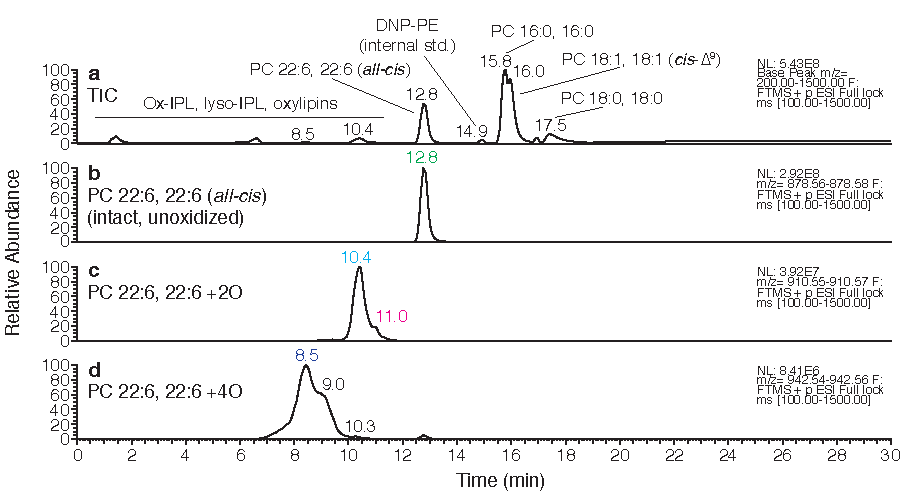
\includegraphics[width=1\textwidth]{Fig_4-8.pdf}
\captionsetup{font={footnotesize}}
\caption[Lipids and oxidized lipids identified in the lipid photooxidation experiment presented in \autoref{fig:c4n6}]{Lipids and oxidized lipids identified in a lipid photooxidation experiment on 14 December 2013. (a) Total ion chromatogram showing all lipids identified in one of three replicate samples of the + UVB -- het. bact. treatment at the final experimental time point (8 h) shown in \autoref{fig:c4n6}. (b)-(d) Extracted ion chromatograms showing the unoxidized PC 22:6, 22:6 parent molecule and two intact oxidized degradation products (ox-PC). Major features are identified by retention time; colored annotations in (b)-(d) correspond to colors used in column headings in \autoref{fig:c4n9} and \autoref{fig:aen4}. Analysis of full-scan and dd-MS\textsuperscript{2} spectra corresponding chromatographically to the different shoulders of the compound peaks in (c) and (d) suggests multiple positional isomers of each species were present in the sample.}
\label{fig:c4n8}
\end{figure}

The results we obtained using the commercial malondialdehyde (MDA) assay kit generally confirmed our other findings. Significantly higher concentrations of MDA were observed in samples of all three light treatments at \emph{t} +8 h compared to the dark control sample sacrificed at the same timepoint (\autoref{fig:c4n6}c). These concentrations (85 $\pm$ 20, 129 $\pm$ 9, and 116 $\pm$ 25 pmol mL\textsuperscript{-1} in the --UVB --het. bact., +UVB --het. bact., and +UVB +het. bact. treatments, respectively; mean $\pm$ SE of three replicates) were of the same order of magnitude as the concentrations of most of the more specific oxidation products we identified in the same samples using our HRAM HPLC-ESI-MS method (\autoref{fig:c4n6}b, \autoref{fig:c4n7}). The elevated concentrations of MDA we observed at the final timepoint in our -- and + UVB treatments, combined with the progressive decrease we observed over time in samples of the dark treatment, suggested new MDA production was supported almost exclusively by photooxidation after decay of the initial concentration present at the outset of the experiment (\autoref{fig:c4n6}c, \emph{t} = 0). We attribute the MDA measured in samples at the initial timepoint to incidental oxidation of PC 22:6, 22:6 and other lipids that occurred during the multiple-hour-long process of liposome preparation. As in the results we recorded for PC 22:6, 22:6 (\autoref{fig:c4n6}a), we noted no significant difference in MDA production in the +UVB +het. bact. treatment compared with the +UVB --het. bact. treatment (\autoref{fig:c4n6}c). Correa-Llant\'{e}n et al. (2012) observed MDA concentrations on the order of $\sim$ 5 nM after exposing a concentrated suspension of PC liposomes to natural UVB radiation; in that study, experimental addition of a photoprotective pigment also demonstrated that lipid photooxidation was significant abiotic source of MDA.

\subsection{Diversity of Photodegradation Products Identified by HRAM HPLC-ESI-MS}
\begin{figure}[!ph]
\centering
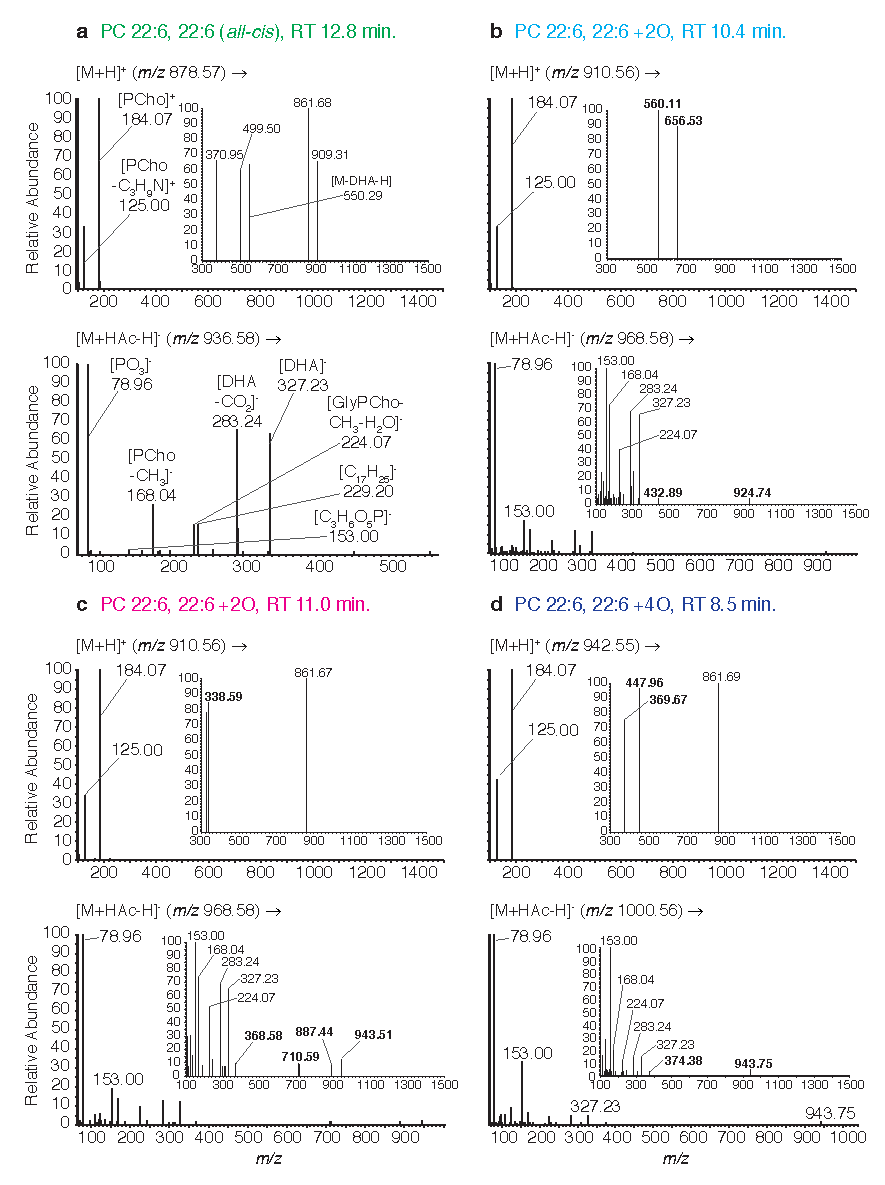
\includegraphics[width=1\textwidth]{Fig_4-9.pdf}
\end{figure}

We used the LOBSTAHS software and several other criteria (described in \autoref{sssec:Chap 4 - Identification and Quantification of Lipids and Oxidized Lipids}, above) to identify lipid degradation products in samples from the experiment presented in \autoref{fig:c4n6}. In the experiment, removal of the unoxidized PC 22:6, 22:6 molecule via photooxidation was accompanied by statistically significant rates of ingrowth of several unoxidized and oxidized derivatives (\autoref{fig:c4n7}, \autoref{fig:c4n8}a; \autoref{table:c4n1}). The former category included significant concentrations of lysophosphatidylcholine (LPC), while the latter included ox-PC species, oxylipins, and several ox-LPC species. The application of an unsupervised clustering algorithm to the data showed that changes in concentration in the various compounds were indicative of expected similarities between both treatments and timepoints (\autoref{fig:c4n7}). While the HPLC-MS data revealed several potential molecules of interest, we focused our efforts on a group of intact oxidized PC (ox-PC) species, a diverse class of molecules which have received increasing attention in human biomedicine (O'Donnell, 2011; Reis and Spickett, 2012; Spickett and Dever, 2005), some terrestrial plant studies (Vu et al., 2012), and other model systems (Ishida et al., 2004), but virtually no attention in oceanography or other avenues of environmental research. While research into the role of oxidized lipids has traditionally focused on the structural diversity and bioactivities of oxylipins --- the short-chain derivatives of fatty acids which are considered the ``terminal'' degradation products of lipid peroxidation processes (Andreou et al., 2009; Cutignano et al., 2011; G\"{o}bel and Feussner, 2009) --- an even broader potential structural and functional diversity exists among larger, more complex intact oxidized PC species and among other oxidized glycerophospholipids (L. T. Morgan et al., 2010; Spickett and Pitt, 2015).

\begin{figure} [!t]
\captionsetup{font={footnotesize}}
\captionof{figure}[Data-dependent MS\textsuperscript{2} spectra of PC 22:6, 22:6 and three oxidized degradation products]{(preceding page) Data-dependent MS\textsuperscript{2} spectra of (a) PC 22:6, 22:6 and (b)-(d) the three oxidized degradation products identified in the + UVB -- het. bact. sample presented in \autoref{fig:c4n8}. The top and bottom plots in each subpanel show, respectively, the positive and negative ionization mode fragmentation spectra for the major adduct of each analyte. Labeled features in (a) are the major ions diagnostic of the intact, unoxidized parent molecule; some of these are diagnostic PC headgroup fragments that also appear in (b)-(d). Boldface \emph{m/}z annotations in (b)-(d) indicate fragment ions unique to each oxidized species. Text colors used in column headings correspond to those used in \autoref{fig:c4n8} and \autoref{fig:aen4}. An expanded version of \autoref{fig:c4n9} is presented in \autoref{fig:aen4}.}
\label{fig:c4n9}
\end{figure}

Analysis of extracted ion chromatograms and data-dependent MS\textsuperscript{2} spectra allowed us to putatively identify a series of progressively more oxidized ox-PC species in a representative +UVB --het. bact. sample at the final experimental timepoint (\autoref{fig:c4n8}, \autoref{fig:c4n9}, and \autoref{fig:aen4}). The accuracy of our mass spectrometer and diagnostic headgroup fragments in the dd-MS\textsuperscript{2} spectra (\autoref{fig:c4n9} and \autoref{fig:aen4}) allowed us to first confirm the identities of these compounds at the level of chemical formula and lipid class. Consistent with the expected effect of increasing molecular polarity on retention time (RT) under reverse-phase chromatographic conditions (O'Donnell et al., 2009), we also observed a decrease in RT of each analyte in the series in proportion to the number of additional oxygen atoms it contained (\autoref{fig:c4n8}b-d; \autoref{table:c4n1}). Further increasing our confidence, an analogous relationship between RT and oxidation state was noted for each of the other types of oxidized species we identified (i.e., ox-LPC and the oxidized free fatty acid derivatives; \autoref{table:c4n1}).

Finally, unique ions observed the MS\textsuperscript{2} spectra for each putatively identified feature (\autoref{fig:c4n9}, S4) indicated either that (a) various positional isomers of each oxidized lipid were present, or (b) the exact nature of the oxidation was different in each case (e.g., the addition of two hydroxyl groups would yields ion of the same \emph{m/z} as one featuring a single hydroperoxy functional group). These unique fragments were distinguished from the common headgroup fragments characteristic of the PC lipid class and other fragments, such as those representing unoxidized DHA, which were present in nearly all of the species (\autoref{fig:c4n9}, S4). Based on previous findings (Milic et al., 2012; O'Donnell, 2011; Reis and Spickett, 2012; Sala et al., 2015; Spickett et al., 2011), we suspect that the apparent diversity of species within each oxidized lipid class reflects a combination of the two situations. We suspect that the compound, non-Gaussian peak shapes we observed for the PC 22:6, 22:6 +2O and PC 22:6, 22:6 +4O species (\autoref{fig:c4n8}c,d) indicate the presence of multiple, near-co-eluting ox-PC regioisomers (i.e., species with same oxidation state and type of oxidized functional group; Domingues et al., 2009; Reis et al., 2005). The presence of multiple isomers of each oxidized species in the sample is highly probable, given the multiple \emph{bis-}allylic positions in the parent molecule and the nonselective, abiotic origin of the peroxidation. Far fewer positional isomers are produced in the case of biologically mediated peroxidation of polyunsaturated fatty acids; this is because the lipoxygenase enzymes responsible for production of short-chain oxylipins tend to have high affinity for specific positions in the acyl chains of their target substrate (Andreou and Feussner, 2009; Brash, 1999; Cutignano et al., 2011; Feussner and Wasternack, 2002).

Because our choice of primary MS method did not yield fragmentation spectra for any of our analytes at levels \textgreater{} MS\textsuperscript{2}, we were unable to further characterize the structures of the ox-PC species we identified in our samples. While fragments diagnostic of specific oxidation types and positions are sometimes observed in the MS\textsuperscript{2} spectra of oxidized phospholipids, spectra obtained from successive fragmentation of target ions at levels \textgreater{} MS\textsuperscript{2} are needed to definitively resolve the structures of many ox-PC species. A significant and growing body of literature offers a wealth of information for analysis of MS\textsuperscript{3} and higher-level data obtained under a variety of HPLC-MS methods in both positive and negative ionization modes (Berliner et al., 2009; Buseman et al., 2006; Domingues et al., 2008; Ishida et al., 2004; Milic et al., 2012; L. T. Morgan et al., 2010; Ni et al., 2015; O'Donnell, 2011; Reis and Spickett, 2012; Sala et al., 2015; Spickett and Dever, 2005; Spickett et al., 2011; Thomas et al., 2010; Yin et al., 2009). Future work will extend the scope of this thesis by examining selected samples on an ion-trap instrument where MS\textsuperscript{n} fragmentation is possible. Authentic standards might also have been used to confirm the identities of some of the species in our samples, but (unlike their shorter-chain molecular cousins, the oxylipins) commercial standards do not exist for the vast majority of ox-PC species. Instead, standards must be obtained either through purification and concentration of fractions from natural samples, or by air oxidation of unoxidized IP-DAG, followed by SnCl\textsubscript{2} reduction and collection of fractions (A. H. Morgan et al., 2010); both of these methods are time-consuming and resource intensive, making the use of ox-PC standards within the scope of the present work prohibitive. The combination of methods we employed still allowed us to make putative identifications of our unknown analytes with a confidence falling somewhere between levels 2 and 3 in the proposed scheme of Sumner et al. (2007) for metabolite identification.

\subsection{Distributions and Acyl Saturation State of IP-DAG in Samples from Waters of the West Antarctic Peninsula}
\begin{figure}[!p]
\centering
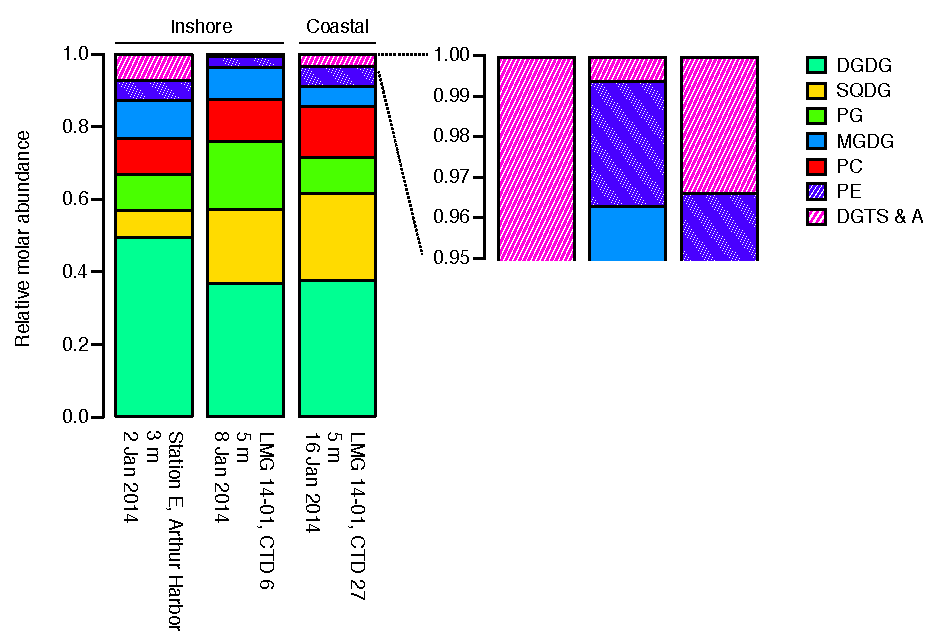
\includegraphics[width=1\textwidth]{Fig_4-10.pdf}
\captionsetup{font={footnotesize}}
\caption[Relative molar distribution of seven classes of IP-DAG in representative samples of particulate biomass from waters of the West Antarctic Peninsula]{Relative molar distribution of seven classes of intact polar diacylglycerol (IP-DAG) in representative samples of particulate biomass (fraction \textgreater{} 0.2 $\mu$m) from waters of the West Antarctic Peninsula. Samples were collected in 2014 from an inshore station (PAL-LTER Station E, 64.82$^{\circ}$ S, 064.055$^{\circ}$ W) and two coastal stations whose biogeochemistry was representative of oceanic influence (cruise LMG 14-01 CTDs 6 and 27, 64.88$^{\circ}$ S, 064.289$^{\circ}$ W and 68.159$^{\circ}$ S, 068.946$^{\circ}$ W, respectively; \autoref{fig:c4n1}). The CTD 6 (8 Jan) sample was obtained during a significant bloom event. Lipids were identified using the LOBSTAHS software (Collins et al., 2016) in conjunction with several additional criteria described in the text; 318 different compounds are represented in the figure. Quantification of lipids was performed using authentic standards. In addition to compounds in the seven lipid classes presented here, we identified several species of diacylglyceryl carboxyhydroxymethylcholine (DGCC) in the samples; these were excluded from the dataset used to generate the figure because we did not have a suitable authentic standard available at the time of analysis. DGCC accounted for \textless{} 11 \% of the total raw IP-DAG peak area in the Station E and CTD 27 samples, and 26.1 \% of the total IP-DAG peak area in the sample from CTD 6. The full, annotated list of the lipids identified in each culture is available online at \url{https://github.com/jamesrco/LipidPhotoOxBox/blob/master/data/nice/LOBSTAHS_lipid_identities/PAL1314_LMG1401_particulate_IP-DAG_pmol_L.final.csv} or upon request from the author.}
\label{fig:c4n10}
\end{figure}

After characterizing the diversity of PC species in HPLC-MS data from our liposome experiments, we applied the same strategy to identify the lipids present in five samples of particulate organic matter ($\geq$ 0.2 $\mu$m) collected from WAP surface waters during the austral spring of 2013-2014. Of the 4,393 different unoxidized and oxidized lipids we identified in the five samples, we used response factors determined from authentic standards to quantify 318 molecules in a subset that encompassed seven different classes of IP-DAG. Triacylglycerols (TAG) accounted for the vast majority (70.0 $\pm$ 8.8 \%, mean $\pm$ SD) of the total identifiable lipid peak area in the five samples. Results from three samples representative of different bloom conditions (\autoref{fig:c4n10} and \autoref{fig:c4n11}) indicated that species of the galactolipid DGDG, one of the four primary IP-DAG in the chloroplast membranes of photosynthetic organisms, accounted for the vast majority of the intact polar lipids we quantified in the data using authentic standards. Significant quantities of the sulfolipid SQDG and the phospholipids PC and PG were also present (\autoref{fig:c4n10}). A comparison of these results with profiles of IP-DAG in four diatom species isolated from WAP waters during the same season (\autoref{fig:aen5}) suggests that other taxa (e.g., heterotrophic bacteria or cryptomonads, which are becoming increasingly prevalent in WAP waters during the spring and summer; Ducklow et al., 2013; Montes-Hugo et al., 2009) contributed equally or more significantly to the surface ocean particulate lipid reservoir during the period. We also identified several oxidized lipid species in the water column samples; these included all of the intact oxidized degradation products of PC 22:6, 22:6 that had we observed in our liposome experiments. Features representing PC 22:6, 22:6 +1O (two obvious isomers), PC 22:6, 22:6 +2O, PC 22:6, 22:6 +3O, and PC 22:6, 22:6 +4O were detected at 7.2, 3.9, 5.1, 0.5, and 0.8 \%, respectively, of the abundance of PC 22:6, 22:6 (percentages are average values across the five samples; a full, annotated list of all identified compounds and their raw chromatographic peak areas are \href{https://github.com/jamesrco/LipidPhotoOxBox/tree/master/data/nice/LOBSTAHS_lipid_identities}{available online}).
\begin{figure}[!p]
\centering
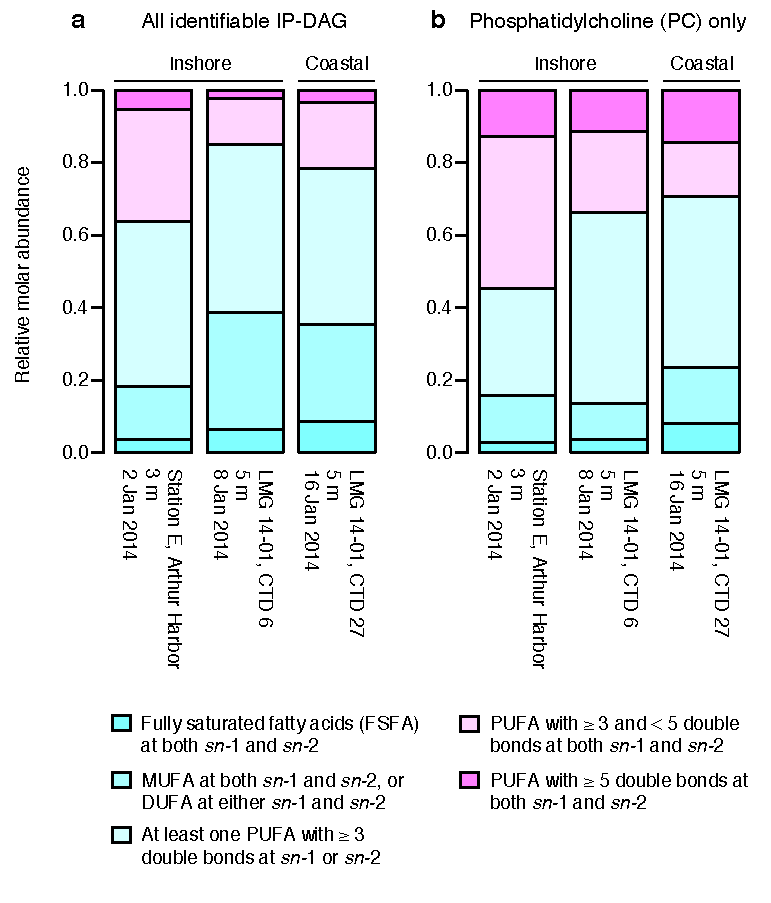
\includegraphics[width=.75\textwidth]{Fig_4-11.pdf}
\captionsetup{font={footnotesize}}
\caption[Fatty acid composition of IP-DAG in the sample presented in \autoref{fig:c4n10}]{Fatty acid composition of (a) all identifiable IP-DAG and (b) phosphatidylcholine (PC) species in the particulate biomass samples presented in \autoref{fig:c4n10}. Because the current version of the LOBSTAHS software resolves the identities of IP-DAG only to the level of bulk fatty acid composition (i.e., the sum of the properties of the substituents at both the \emph{sn}-1 and \emph{sn}-2 positions), we were unable to determine which fatty acids were present in each molecule without significant additional inspection of fragmentation spectra or saponification for analysis of fatty acid methyl esters (FAMES). However, we were able to categorize the saturation state of the IP-DAG according to the simplified scheme we present here after verifying (by inspection of fragmentation spectra) that the maximum degree of unsaturation of any single fatty acid present in these species was six (present in the form of docosahexaenoic acid, or DHA).}
\label{fig:c4n11}
\end{figure}

As a second means of analysis with direct relevance to the project described in this chapter, we binned the IP-DAG species in each water column sample into five categories based on the saturation state of their attached fatty acids (\autoref{fig:c4n11}). Molecular species containing highly polyunsaturated fatty acids (i.e., those with $\geq$ 5 double bonds) at both substituent positions accounted for 5.3, 2.3, and 3.4 \% of the IP-DAG in samples from PAL-LTER Station E and LMG 14-01 CTD stations 6 and 27, respectively (percentages calculated on basis of molar concentration; \autoref{fig:c4n11}a). Lipids containing two fatty acids of moderate polyunsaturation (i.e., $\geq$ 3 but \textless{} 5 double bonds) accounted for 31.1, 12.7, and 18.2 \% of IP-DAG in the three samples. When we examined the acyl saturation state of molecular species belonging to single classes of IP-DAG, it became apparent that PUFA were not evenly distributed throughout the WAP metalipidome (e.g., PUFA were concentrated more heavily in species of PC than in the IP-DAG pool as a whole; \autoref{fig:c4n11}b). Comparison of these results with a similar analysis of fatty acid distribution among IP-DAG classes in the four diatom isolates (\autoref{fig:aen6}) again showed that the lipids of these diatoms did not dictate the composition of the overall WAP lipid pool, despite these species being traditionally responsible for most early-season blooms in WAP waters.

\section{Discussion}
\subsection{Apparent Dependence of Photolability on Acyl Polyunsaturation}
\label{ssec:Apparent Dependence of Photolability on Acyl Polyunsaturation}

PC 22:6, 22:6 was the only species we evaluated that contained polyunsaturated fatty acids (PUFA) with more than two double bonds (\autoref{table:aen1}; molecular structures, \autoref{fig:aen1}). Our laboratory measurements of decadic molar absorptivity show that the capacity of PC 22:6, 22:6 to absorb light in both the UVB and UVA spectral bands exceeded by nearly two orders of magnitude those of direct molecular analogs containing fully saturated (PC 22:0, 22:0) and monounsaturated (PC 22:1, 22:1) fatty acids of the same chain length (\autoref{fig:c4n5}c). The large difference we observed between the molar absorptivity of the hexa-unsaturated compound and its more saturated analogs was corroborated by similar results previously reported for other sequences of related phospholipids (McHowat et al., 1996; Spector et al., 1996). In addition, UV-visible absorbance measurements of docosahexaenoic acid, the constituent fatty acid of PC 22:6, 22:6, indicated that the parent molecule's light-absorbing capacity was due primarily to the presence of the highly unsaturated acyl moiety and not the polar headgroup (\autoref{fig:c4n5}b,c). Absorbance measurements of the lipid standards were repeated for verification in three independent experiments over the course of two months. While no molar absorptivity data have been published for PC 22:6, 22:6, the ${\varepsilon _i}(\lambda )$ we calculated for DHA agreed generally with values found in the literature (Whitcutt, 1957). In the only investigation directly analogous to the work in this thesis chapter, R. J. Kieber et al. (1997) investigated the photochemical reactivity of highly polyunsaturated free fatty acids in seawater under exposure to natural sunlight. In that study, photodegradation rates of C\textsubscript{16} and C\textsubscript{18} PUFA were nearly 10 times those of the species' monounsaturated counterparts and --- perhaps most instructively for purposes of interpreting the present results --- the investigators observed almost no photodegradation in the saturated member of the C\textsubscript{16} series, palmitic acid. Rontani et al. (1998) observed a similar trend for a series of C\textsubscript{18:1}-C\textsubscript{18:3} fatty acids isolated from algal cultures; while that experiment did not include any PUFA with more than three double bonds, the degradation rate constant the authors observed for the C\textsubscript{18:3} species was more than six times that observed for C\textsubscript{18:1}.

While Wagner et al. (1994) did not specifically investigate the \emph{photochemical} lability of fatty acids, they hypothesized that the ``oxidizability'' of a given PUFA --- the overall susceptibility of its hydrogen atoms to abstraction by radical species such as $\bullet$OH --- was proportional not simply to the number of double bonds in the fatty acid, but to the number of \emph{bis-}allylic positions in the fatty acid chain. Applying this hypothesis in a series of experiments, the authors found that the addition of each new double bond which created a \emph{bis-}allylic carbon atom increased exponentially the rate at which a given fatty acid was oxidized. The bond dissociation energy of a doubly allylic C-H bond was reported to be just 314-335 kJ mol\textsuperscript{-1}, compared with 368 kJ mol\textsuperscript{-1} for a singly allylic bond and 423 kJ mol\textsuperscript{-1} for an alkyl C-H bond (Gardner, 1989; Koppenol, 1990).

\subsubsection{Other Sources of Evidence for Preferential Photooxidation of PUFA-Containing Lipids}

Beyond the previous results we reviewed in in the above paragraphs (\autoref{ssec:Apparent Dependence of Photolability on Acyl Polyunsaturation}), we could find no empirical evidence in the literature for a quantitative relationship between IP-DAG molecular structure (specifically, the degree of acyl unsaturation) and photochemical lability in the environment or under environmentally relevant experimental conditions. Several lines of evidence generally substantiate the enhanced photochemical lability of acyl lipids bearing polyunsaturated fatty acids over closely related molecules with lower degrees of unsaturation. First, an extensive body of research spanning diverse scientific disciplines has long ranked polyunsaturated fatty acids among the cellular lipid components most susceptible to photooxidation (Girotti, 1990; Heath and Packer, 1968; Rontani, 1999) and transformation by reactive oxygen species (ROS) generally (Frankel, 1980; 1987; Girotti, 1998; Li and Schwarz, 2012; Mene-Saffrane et al., 2009). Some evidence for a quantitative relationship between acyl unsaturation and photochemical lability in IP-DAG exists in human biomedicine, where artificial near-IR radiation can be used to trigger release of pharmaceutical compounds from liposomes for targeted, intracellular drug delivery. In one study that investigated the intracellular release of a cancer chemotherapy medication encapsulated in PC liposomes, a quantitative, negative relationship was observed between the degree of unsaturation of the fatty acids used in the liposomes and the time required to achieve 50 \% release of the drug into the cell (Luo et al., 2016). Earlier work (Pashkovskaya et al., 2010) suggested the mere presence of unsaturated acyl moieties could dramatically enhance the apparent photochemical lability of the entire liposome pool used for drug delivery, a finding consistent with evidence that autooxidation of saturated lipid moieties can be initiated by lipid radicals derived from oxidation of nearby PUFA (Girotti, 1998).

Of course, there is abundant evidence from incubation experiments with both single-species cultures and whole communities of phytoplankton that PUFA are preferentially underexpressed in marine microorganisms that are subjected to high doses of UV radiation (Hessen et al., 1997). Whether this is predominantly because cell membranes containing these PUFA are abiotically oxidized at a greater rate under UV radiation, or because UV radiation inhibits the organisms' ability to synthesize these critical compounds is not clear; both mechanisms appear to be important (Goes et al., 1994). Hessen et al. (1997) and Wang and Chai (1994) both noted that phytoplankton membrane lipids containing eicosapentaenoic acid (EPA, 20:5$\omega$3) and DHA were particularly susceptible to photooxidation, confirming our results in the present study (\autoref{fig:c4n6}a; \autoref{table:c4n1} and \autoref{table:aen1}); Wang and Chai found that an acute dose of strong UVB radiation elicited a stronger response than application of a less intense dose over a longer time period. After exposing cultures of three Antarctic marine phytoplankton to different levels of UVB radiation, Skerratt et al. (1998) found some evidence that UVB exposure could reduce intercellular ratios of unsaturated to saturated fatty acids; however, the response to UVB exposure was species-specific and depended heavily on the dosage. For example, while the ratio of PUFA : FSFA remained virtually unchanged in the diatom \emph{Odontella weissflogii} after two days of exposure to elevated concentrations of UVB radiation, the percentage of total fatty acids identified as PUFA in the diatom \emph{Chaetoceros simplex} decreased from 37 to 31 \%. Guih\'{e}neuf et al. (2010) also noted that the response of different phytoplankton species to UVB radiation appeared highly species specific, observing significant reductions in EPA and DHA-containing phospho- and glycolipids in one species (\emph{Pavlova lutheri}) yet very little change in another (\emph{Odontella aurita}).

\subsection{Possible Mechanisms Supporting Observed Rates of Photooxidation}

Although the original scope of this chapter did not extend to identification of the mechanism(s) responsible for the photooxidation we observed in the liposome experiments, several conclusions can be drawn from synthesis of available environmental and optical data, the results of two \emph{ad hoc} experiments, and previous findings regarding photochemical processes in waters of the WAP and other polar marine ecosystems. First, our results show that photooxidation could have been supported by both indirect (i.e., via ROS produced through reactions with chromophoric substances) and direct (i.e., via the action of a photon directly upon a molecule) processes. We observed penetration through nearly the entire mixed layer (see \autoref{ssec:Irradiance Observations; UV Penetration Through Shallow Mixed Layer}, above) of significant radiation in both the UVA and UVB spectral bands, indicating ample photons were available in the surface water column to initiate or catalyze a variety of reactions; nearly 70 \% of incident UVB radiation (\autoref{fig:c4n3}a and \autoref{fig:c4n4}) and 40 \% of UVA radiation (\autoref{fig:c4n3}b and \autoref{fig:c4n4}) were observed to reach a depth of 0.6 m. Based on the abundance of UVA radiation in the water column and the 314-335 kJ mol\textsuperscript{-1} bond energy previously reported for the doubly allylic C-H bonds in model PUFA (Gardner, 1989; Koppenol, 1990), we suggest direct photolysis of PC 22:6, 22:6 could have contributed significantly to overall rates of PUFA photooxidation throughout much of the shallow surface layer. The 314-335 kJ mol\textsuperscript{-1} bond energy is equivalent to that carried by UVA-band photons of $\lambda$ between 357 and 381 nm; quanta of this energy were abundant to depths of at least 8 m in the waters of Arthur Harbor (\autoref{fig:c4n4}).

Of the many possible indirect mechanisms that could have supplemented direct photolysis in immediate surface waters during the period of our study, the generation (and peroxidation thereby) of hydroxyl radical from photoexcitation of existing nitrate and nitrite stocks was almost certainly significant. Qian et al. (2001) found that UVA + UVB excitation of DOM, combined with UVB excitation of relatively high NO\textsubscript{3}\textsuperscript{-} concentrations often typical of Southern Ocean waters, led to enhanced rates of $\bullet$OH production in surface waters of the WAP. While we did not measure production rates or steady-state concentrations of $\bullet$OH in the present study, the daily doses of UVB radiation received at Palmer Station in the spring of 2013 were similar to those received on many days during the season in which Qian et al. conducted their study. Furthermore, in 2013-2014, surface concentrations of NO\textsubscript{3}\textsuperscript{-} + NO\textsubscript{2}\textsuperscript{-} remained at or above 15 $\mu$M at PAL-LTER Stations B and E until early January, providing a sufficient reservoir of the chromophore to sustain production of hydroxyl radical at biogeochemically significant rates (public PAL-LTER data; not shown). While a combined concentration of the two nutrients of just 1.2 $\mu$M was measured at Station E following a bloom event in mid-January, concentrations at both stations increased again soon after the event to yield a seasonal average of 15.0 $\mu$M at depths \textless{} 5 m. The ability of $\bullet$OH to abstract hydrogen atoms from PUFA has been well-demonstrated (Porter et al., 1995; Wagner et al., 1994) and we therefore do not devote additional discussion to the topic here.

While photochemical generation of other ROS such as \textsuperscript{1}O\textsubscript{2}, H\textsubscript{2}O\textsubscript{2}, and O\textsubscript{2}\textsuperscript{-} might certainly have augmented the two photochemical sinks we discuss in the paragraph above, we believe it unlikely that photochemically produced H\textsubscript{2}O\textsubscript{2} and O\textsubscript{2}\textsuperscript{-} contributed significantly to overall rates of lipid degradation in our experiments. Photoexcitation in the laboratory of previously frozen, 0.7 $\mu$m-filtered water samples from Arthur Harbor (the experiments described in \autoref{ssec:Laboratory Determination of ROS Photoproduction and Decay}) yielded negative results at all wavelengths; photoproduction rates of H\textsubscript{2}O\textsubscript{2} and O\textsubscript{2}\textsuperscript{-} remained below detection in all instances. We still could not detect any superoxide after spiking the sample with 10-200 nM KO\textsubscript{2}; this suggested the seawater contained a strong abiotic quenching agent capable of scavenging the two ROS. However, the outcome of this brief experiment is challenged by the findings of both Yocis et al. (2000), who measured H\textsubscript{2}O\textsubscript{2} photoproduction rates of 2.1 to 9.6 nM H\textsubscript{2}O\textsubscript{2} hr\textsuperscript{-1} in fresh, unfiltered West Antarctic waters, and of Kieber et al. (2014), who made similar findings. Thus, a biological source of H\textsubscript{2}O\textsubscript{2} might have contributed to rates of lipid oxidation in natural waters outside of our experimental construct; water column concentrations of 10-100 nM H\textsubscript{2}O\textsubscript{2} were observed at Palmer Station during the 2015-2016 field season (although, H\textsubscript{2}O\textsubscript{2} concentrations in dense algal biomass were as high as 200 nM; J. Bowman, \emph{Pers. comm.}). The 2015-2016 water column concentrations were consistent with the concentrations measured in surface waters at several offshore PAL-LTER stations during the early 1990s (12-21 nM; Resing et al., 1993). We did not make measurements of singlet oxygen in the course of this work, and it is likely the species contributed significantly to the rates of photooxidation we report here. Type II (i.e., \textsuperscript{1}O\textsubscript{2}-mediated) photooxidation of lipids has been proposed as the dominant pathway for photooxidation in marine systems of monounsaturated fatty acids and photosynthetic pigments (Rontani, 1999)

\subsection{Biogeochemical Significance of Lipid Photooxidation in Surface Waters of the West Antarctic Peninsula}
\subsubsection{Choice of Apparent Quantum Yield for Use in Calculations}

Using the oxidation rates we obtained from our liposome experiments and several other measured properties, we calculated three broadband polychromatic AQY for photooxidation of PUFA-containing IP-DAG in coastal waters of West Antarctica (\autoref{table:c4n2}). Uncertainities were determined as described in \autoref{sssec:Determination of Uncertainties in AQY Estimates}. Based on our findings that UVB radiation did not significantly enhance rates of photooxidation in PUFA-containing IP-DAG beyond those rates observed in the presence of UVA radiation alone (\autoref{fig:c4n6}; \autoref{table:c4n1}), we chose to apply in our subsequent calculations the broadband AQY ${\Phi _{UVA}}$, which parameterizes the photooxidation rate as a function of the total radiation received in the UVA spectral band. Our laboratory measurements confirmed the capacity of PC 22:6, 22:6 to absorb light over a broad wavelength range that extended far into the UVA spectrum (\autoref{fig:c4n5}). Because we could find no AQY (polychromatic or otherwise) in the literature for IP-DAG or polyunsaturated fatty acids, the best empirical evidence outside the present study comes from the rate constants calculated by Christodoulou et al. (2010), Rontani et al. (1998), and others. In applying a yield that accounts for multiple processes operating across a wide spectrum, we proceed from the conclusion of the former authors, who found that maximum degradation rates of polyunsaturated lipids in senescent phytoplanktonic cells were induced by both a combination of visible light (photosynthetically active radiation wavelengths) and UVA radiation. To obtain a conservative estimate of the possible impact of lipid photooxidation on the organic matter inventory in surface waters of the West Antarctic Peninsula, we applied our broadband AQY to the most polyunsaturated fraction of the IP-DAG identified in our water column samples (\autoref{fig:c4n11}). For comparison, we made a series of parallel calculations in which we applied the same AQY to the larger, moderately polyunsaturated fraction of the IP-DAG inventory. We assumed in our calculations that the residence times of suspended and slowly sinking particulate organic matter in the mixed layer were long (i.e., on timescales of days) compared with the timescale over which photodegradation was observed to act in our liposome experiments (i.e., 8.2-12.4 hr).
\begin{figure}[!p]
\centering
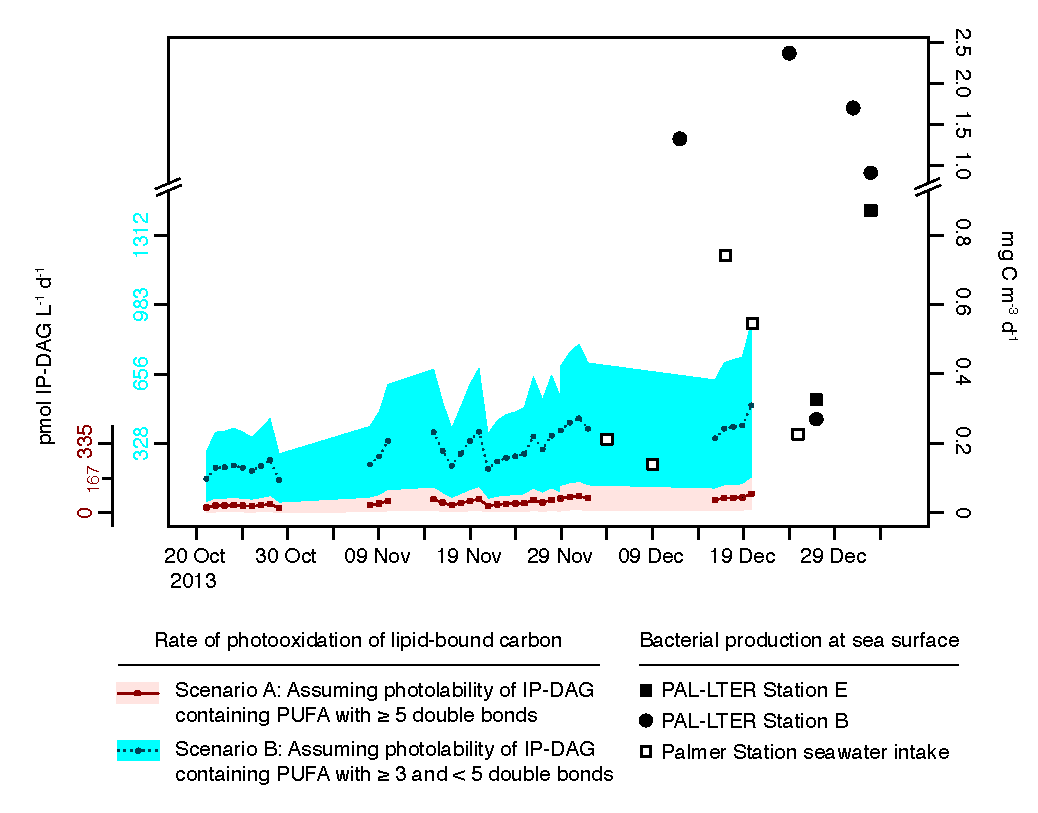
\includegraphics[width=1\textwidth]{Fig_4-12.pdf}
\captionsetup{font={footnotesize}}
\caption[Potential rates of lipid photooxidation in particulate organic matter of West Antarctic Peninsula surface waters]{Potential rates of lipid photooxidation in particulate organic matter of West Antarctic Peninsula surface waters over a 2-month period in the austral spring of 2013. High-resolution, \emph{in situ} time-series observations of downwelling irradiance and a broadband polychromatic apparent quantum yield (AQY) for IP-DAG species containing highly polyunsaturated fatty acids (${\Phi _{UVA}}$) were applied to separate fractions of lipids identified using the LOBSTAHS software to generate two sets of photooxidation rate estimates. In the first, most conservative scenario (red markers and solid trace), we applied the irradiance time series and AQY to only those IP-DAG containing PUFA with $\geq$ 5 double bonds at both the \emph{sn}-1 and \emph{sn}-2 backbone positions. In the second, more permissive scenario (cyan markers and dashed trace), we assumed the AQY could also be applied to molecular species containing PUFA with $\geq$ 3 but \textless{} 5 double bonds. ${\Phi _{UVA}}$ represents the reaction yield for lipid photooxidation based on the quantity of UV radiation received between 315 to 395.5 nm; estimation of ${\Phi _{UVA}}$ and the associated uncertainty is described in \autoref{ssec:Calculation of Broadband Polychromatic Apparent Quantum Yields (AQY)} of the text. The shaded regions represented the propagated uncertainties in each estimate determined using a series of Monte Carlo simulations. Lipid photooxidation rates (left-hand \emph{y-}axis) were converted units of mg C m\textsuperscript{-3} d\textsuperscript{-1} based on the mean carbon content of the IP-DAG identified in each unsaturation fraction; these were 49. 3 $\pm$ 0.5 and 50.6 $\pm$ 0.6 mol C : mol lipid for the polyunsaturated (cyan) and highly polyunsaturated (red) fractions, respectively. Presented for comparison are volumetric rates of bacterial production for West Antarctic Peninsula surface waters, obtained using the \textsuperscript{3}H-leucine incorporation method (large individual symbols, from PAL-LTER data; Bowman et al., 2016). Note the break and change in scale of the \emph{y-}axis.}
\label{fig:c4n12}
\end{figure}
\subsubsection{Photooxidation Rates in Austral Spring of Same Order of Magnitude as Bacterial Production}

Our results (\autoref{fig:c4n12}) suggest that photooxidation of IP-DAG containing highly polyunsaturated fatty acids represents a biogeochemically significant process in this ecosystem of a magnitude commensurate with that of bacterial production. While limiting the scope of our findings to the early spring --- when nearly all of the suspended particulate biomass in the shallow mixed layer receives enhanced doses of UV radiation through a depleted stratospheric ozone layer --- we estimate conservatively that, on average, 52 $\pm$ 12 pmol IP-DAG m\textsuperscript{-3} d\textsuperscript{-1} was oxidized in the mixed layer by photochemical processes (this is the equivalent of 0.032 $\pm$ 0.007 mg C m\textsuperscript{-3} d\textsuperscript{-1}; \autoref{fig:c4n12}, red markers and solid red trace). Under the second, less conservative scenario --- in which we applied the AQY to a larger subset of the IP-DAG inventory --- we estimate that roughly 6 times this quantity of lipid organic matter was potentially oxidized through photochemical mechanisms (307 $\pm$ 69 pmol IP-DAG m\textsuperscript{-3} d\textsuperscript{-1}, equivalent to 0.18 $\pm$ 0.04 mg C m\textsuperscript{-3} d\textsuperscript{-1}; \autoref{fig:c4n12}, cyan markers and dashed trace). For comparison, average surface ($\leq$ 5 m) rates of bacterial production at the three PAL-LTER stations in the period before 4 January 2014 were 0.38 $\pm$ 0.26, 1.3 $\pm$ 0.8, and 0.60 $\pm$ 0.4 mg C m\textsuperscript{-3} d\textsuperscript{-1} (Palmer Station seawater intake, PAL-LTER Station B, and PAL-LTER Station E, respectively, assuming a conversion factor of 1.5 kg C (mol leucine)\textsuperscript{-1} and isotope dilution of 1; \autoref{fig:c4n12}, larger symbols). We thus calculate that, during the early spring, lipid photooxidation might represent a flux of between 2-8 \% (conservative scenario) or 14-47 \% (alternative scenario) of the strength of bacterial carbon metabolism in WAP surface waters. We suspect that even our less conservative calculations might still represent an underestimate of the overall significance of lipid photooxidation in WAP waters because we did not apply our model to any fraction of the lipid biomass allocated to triacylglycerols, which accounted for 70-75 \% of the total identifiable chromatographic peak area in the water column samples. Although the AQY was derived from photooxidation experiments in PC, we justify its application to other classes of IP-DAG on the basis of evidence (from human systems) that changes in headgroup do not dramatically affect \emph{in situ} oxidation rates so long as the attached PUFA are of high unsaturation (Reis and Spickett, 2012).

We converted our photooxidation rate estimates from units of lipid (i.e., pmol IP-DAG m\textsuperscript{-3} d\textsuperscript{-1}) to carbon based on the carbon content of the IP-DAG identified in each unsaturation fraction; these were 49. 3 $\pm$ 0.5 and 50.6 $\pm$ 0.6 mol C : mol lipid for the polyunsaturated (cyan) and highly polyunsaturated (red) fractions, respectively. In doing so, we assumed that photooxidation of given lipid would in most instances lead to the eventual remineralization of the molecule's constituent carbon. Because lipid peroxidation proceeds by a free radical chain reaction mechanism (Girotti, 1990; Halliwell and Chirico, 1993), we assumed that, in the environment, the vast majority of initial oxidation products --- such as the ox-PC we have identified in this study --- would further degrade into smaller molecular components, while also initiating the degradation of other nearby lipids (and other molecules) that contain easily abstracted hydrogen atoms (Crastes de Paulet et al., 1988). The significant fraction of these smaller molecules that enter the dissolved organic matter pool will remain near the ocean's surface where, as previous work has demonstrated, they may be oxidized abiotically to dissolved inorganic carbon (Miller and Zepp, 1995). Equally as likely, these smaller, more labile molecules may be assimilated and remineralized by heterotrophic bacteria in the water column; this fate is support by considerable previous work (reviewed in D. J. Kieber, 2000) and our findings in \autoref{sssec:Some Support for Bacterial Metabolism of Oxidized Degradation Products}. However, we acknowledge here the many adaptations to oxidative stress possessed by phytoplankton, including considerable capacity to dissipate ROS and dozens of mechanisms for repair of damage to oxidized biomolecules (Roy, 2000). It is thus possible, as Rontani et al. (2016) have suggested based on observations in the Arctic, that the lipids in living phytoplankton cells may be much less susceptible to photooxidation than lipids in senescent or dead biomass. We do note that in the 2016 study, Rontani et al. did not look for evidence of photooxidation in intact lipids (i.e., ox-IPL) or in the oxidized products of lipids containing fatty acids with more than one double bond.

Our results nevertheless suggest that the shallow mixed layers which can form in the marginal ice zone provide a sort of ``optical incubator'' for UVR-induced lipid peroxidation in the WAP. In this model, particulate organic matter, including both ice-attached and free-living phytoplankton and bacteria, is exposed for extended periods to intense UV radiation at the immediate sea surface, increasing photooxidation rates of photolabile compounds such as PUFA-containing IP-DAG. Rontani et al. (2016) applied a version of this model to a recent analysis of lipid biomarkers in surface-layer biomass and shallowly deployed sediment traps (5 and 30 m) at the MIZ in the Canadian Arctic, finding that extended exposure to UVR of slowly-sinking aggregates derived from senescent sea-ice algae left a strong imprint on the photodegradation state of the lipid pool.

\subsection{Future Implications for the West Antarctic Peninsula Marine Ecosystem}

Three significant, relatively recent changes in the ecosystem of the West Antarctic Peninsula (Ducklow et al., 2013; Saba et al., 2014) make it difficult to predict how (or whether) lipid photooxidation will impact rates of primary production or carbon export in the future. First, shifts in the species composition of the phytoplankton community responsible for primary production in waters of the West Antarctic Peninsula --- particularly, increases in the prevalence of cryptophytes (or cryptomonads; phytoplankton of the phylum Cryptophyta) at the expense of the diatoms traditionally responsible for most of the carbon fixation (Montes-Hugo et al., 2009) --- will likely drive shifts in the lipid composition of surface ocean biomass during and after the annual retreat of the sea ice. While much is known about the lipid profiles of diatoms generally and species native to Antarctica in particular (e.g., \autoref{fig:aen5} and \autoref{fig:aen6}), relatively little comparable data exists for cryptophytes, apart from a few select species which have been investigated extensively for their potential as a feedstock for biodiesel production. DGDG is the most abundant IP-DAG in at least one cryptophyte, \emph{Chroomonas salina} (Henderson and Mackinlay, 1989).

Second, should the significant warming of WAP waters that has been observed in recent decades continue (Ducklow et al., 2013), the increase in average sea surface temperature could drive changes in the saturation state of the marine lipid pool independent of any change attributable to shifts in species distribution. Experimental results in cultures of several different marine phytoplankton species show that even modest increases in temperature can drive significant decreases in the proportion of overall membrane lipids that contain polyunsaturated fatty acids (Guschina and Harwood, 2006). This general relationship between saturation state and temperature has been demonstrated specifically in cultures of \emph{C. salina} (Henderson and Mackinlay, 1989). While the lipid inventories at several sites along the West Antarctic Peninsula presently include robust concentrations of IP-DAG with sufficient PUFA to support biogeochemically significant rates of photooxidation (\autoref{fig:c4n11} and \autoref{fig:c4n12}), warmer waters and an ecological shift toward phytoplankton species of largely uncharacterized lipid composition could alter the significance of photooxidation in the ecosystem.

Third, reductions in the duration and extent of sea ice cover that have accompanied the increase in WAP sea surface temperatures (Meredith and King, 2005) will likely diminish the strength of ice-associated and ice-attached diatom communities and their relative contribution to the overall lipid pool. The lipids produced by ice-attached diatom communities are different in many ways from those produced by diatoms which make their living in the water column (Fahl and Kattner, 1993; Falk-Petersen et al., 1998; Mock and Kroon, 2002). Because primary production in WAP waters is typically distinguished by bloom events that begin at the receding sea ice edge in spring or early summer (Ducklow et al., 2013; Vernet et al., 2008), warming water and concomitant changes in annual sea-ice dynamics could also advance the timing of blooms to earlier in spring and shift their locations further south, which could lead to ever greater temporal and spatial coincidence between maximum UVR exposure and peak phytoplankton abundances. A final, more recent trend --- the reduction in the size of and severity of the seasonal ozone anomaly over Antarctica, driven by recovery in stratospheric O\textsubscript{3} stocks (Solomon et al., 2016) --- could represent a significant negative feedback on photooxidation, further complicating any attempt to predict the overall significance of the process in a future ecosystem state.

\section{Conclusions and Additional Biogeochemical Implications}

While we show here that lipid photooxidation is a biogeochemically significant process that can impact the turnover of carbon in the surface ocean on scales commensurate with bacterial remineralization, it was ultimately beyond the scope of this thesis to determine whether the photooxidation of lipids containing polyunsaturated fatty acids leaves any significant imprint on the quality or the magnitude of organic matter exported to the ocean's depths. While we did not observe statistically significant rates of photooxidation in monounsaturated IP-DAG, a significant body of literature has shown that MUFA-derived oxylipins (i.e., free fatty acid derivatives cleaved from their lipid headgroup) do contribute to the oxidized lipid pool in surface waters, sinking particles, and seafloor marine sediments on scales which are all environmentally relevant (Marchand and Rontani, 2001; Rontani, 1999; Rontani et al., 2016; Rontani et al., 2012a; Rontani et al., 2012b). In Antarctic waters specifically, there is reason to presume that oxidation and removal of certain lipids at the ocean's surface could affect the quality of the lipid biomass that is exported to depth. Hayakawa et al. (1996) used a moored sediment trap at a site in Breid Bay, East Antarctica (trap depth 111 m; water depth 300 m) to examine the fatty acid content of sinking particles at 3.5-day intervals over three months, finding that the composition of the material bore the direct imprint of biogeochemical events at the ocean's surface. PUFA accounted for an average of 8.6 \% of fatty acids in all samples collected over the course of the study, but \textgreater{} 16 \% of the total during two diatom blooms which were observed at the site in the austral spring. EPA (20:5$\omega$3) alone accounted for 7.3 and 9.1 \% of the total during the two bloom events. Of course, one must also consider the possible impact that UV-induced PUFA photooxidation (and/or suppression of PUFA biosynthesis) in living phytoplankton might have for grazing zooplankton and, in turn, higher trophic level consumers. Ha et al. (2014) found that experimentally-induced reductions in the PUFA quotient of lipids in a sub-Antarctic natural phytoplankton assemblage --- particularly, reductions in the concentrations of DHA and EPA --- were passed in part to amphipods that fed on the phytoplankton deficient in essential fatty acids.

Finally, this study does not even begin to address the diversity of possible infochemical impacts that the many new oxidized phospholipid compounds we putatively identify (\autoref{fig:c4n7}, \autoref{fig:c4n8}, \autoref{fig:c4n9}, and \autoref{fig:aen4}) might have on intracellular processes, interactions between microoorganisms in the water column, or on the remineralization of sinking marine particles. Edwards et al. (2015) demonstrated the significant impact that modest concentrations of a single class of well-characterized oxylipin could have on the rate at which sinking marine particles were remineralized; given the hundreds of other oxylipins and many different intact oxidized phospholipids with significant known or hypothesized bioactivities in humans (Reis and Spickett, 2012; Spickett and Dever, 2005; Spickett and Pitt, 2015) and terrestrial plants (Vu et al., 2012), it is highly probable that some of these same compounds or their close analogs must play similar or as-yet-unimagined roles in the ocean.

\section{Acknowledgements}

We thank the captains, crew, and science support staff of the ARSV \emph{Laurence M. Gould}, the science support staff at Palmer Station during the 2013-2014 and 2015-2016 field seasons, and many current and former PAL-LTER team members for assistance with field sampling and sample analysis. We thank Jeff Bowman, Ollie Zafiriou, and Collin Ward for various discussions that focused our hypotheses and sampling plan. We also thank Kevin Becker, Peter Blandori, Nicole Couto, Julia Diaz, Scott Doney, Bethanie Edwards, Matthew Erickson, Tina Haskins, Meredith Helfrich, Oliver Ho, Fiona Hopewell, Carolyn Lipke, Austin Melillo, Justin Ossolinski, Naomi Shelton, Jeremy Tagliaferre, and Sebastian Vivancos for various analytical and logistical assistance. Oligotrophic seawater from the BATS site was kindly provided by Dan Repeta. Assistance with data from the Antarctic Ultraviolet Monitoring Network was provided by Patrick Disterhoft and the radiation group of NOAA's Global Monitoring Division, 325 Broadway, Boulder, CO, 80303. J.R.C. acknowledges support from a U.S. Environmental Protection Agency (EPA) STAR Graduate Fellowship (Fellowship Assistance agreement FP-91744301-0). The contents of this research have not been formally reviewed by EPA. The views expressed in this manuscript are solely those of the authors, and EPA does not endorse any products or commercial services mentioned therein. This work was also supported by U.S. National Science Foundation award OCE-1059884 to B.A.S.V.M., the Gordon and Betty Moore Foundation through grant GBMF3301 to B.A.S.V.M., and a WHOI Ocean Ventures Fund award to J.R.C. The field work conducted at Palmer Station and aboard the ARSV \emph{Laurence M. Gould} was supported by the Palmer LTER study (U.S. NSF awards OPP-9011927, 9632763, 0217282, 0823101, and GEO-PLR 1440435).

\section{Availability of Data, Code, and Supplementary Methodological Details}

The R scripts and processed data files required to reproduce the results and figures in this work are available online at \url{https://github.com/jamesrco/LipidPhotoOxBox}. Methodological details, additional figures, and an additional table, are included as supporting information. All PAL-LTER data used in this manuscript were downloaded from the Palmer LTER Datazoo at \url{http://oceaninformatics.ucsd.edu/datazoo/data/pallter/datasets}. Raw MS data files (\textgreater{} 200 MB) and raw spectral data collected using the Jaz instrument are available upon request from the author. Processed MS data, aggregated Jaz spectra, and detailed protocols for liposome preparation and the exoenzyme assays are available via the GitHub link above. NOAA spectroradiometer data were downloaded from \url{http://www.esrl.noaa.gov/gmd/grad/antuvdata/}.
\clearpage
\begin{singlespace}
\section*{References}
\addtocounter{section}{1}
{\setlength{\parindent}{0pt}
Andreou, A., and I. Feussner (2009), Lipoxygenases - Structure and reaction mechanism, \emph{Phytochemistry}, \emph{70}(13-14), 1504-1510, doi:\href{http://dx.doi.org/10.1016/J.Phytochem.2009.05.008}{10.1016/J.Phytochem.2009.05.008}.

{\setlength{\parskip}{10pt}

Andreou, A., F. Brodhun, and I. Feussner (2009), Biosynthesis of oxylipins in non-mammals, \emph{Progress in Lipid Research}, \emph{48}(3-4), 148-170, doi:\href{http://dx.doi.org/10.1016/J.Plipres.2009.02.002}{10.1016/J.Plipres.2009.02.002}.

Armstrong, D., and R. Browne (1994), The analysis of free radicals, lipid peroxides, antioxidant enzymes and compounds related to oxidative stress as applied to the clinical chemistry laboratory, in \emph{Free Radicals in Diagnostic Medicine: A Systems Approach to Laboratory Technology, Clinical Correlations, and Antioxidant Therapy}, edited by D. Armstrong, pp. 43-58, Springer US, Boston, MA, doi:\href{http://dx.doi.org/10.1007/978-1-4615-1833-4_4}{10.1007/978-1-4615-1833-4\_4}.

Barofsky, A., and G. Pohnert (2007), Biosynthesis of polyunsaturated short chain aldehydes in the diatom \emph{Thalassiosira rotula}, \emph{Organic Letters}, \emph{9}(6), 1017-1020, doi:\href{http://dx.doi.org/10.1021/ol063051v}{10.1021/ol063051v}.

Benton, H. P., E. J. Want, and T. M. D. Ebbels (2010), Correction of mass calibration gaps in liquid chromatography-mass spectrometry metabolomics data, \emph{Bioinformatics}, \emph{26}(19), 2488-2489.

Berliner, J. A., N. Leitinger, and S. Tsimikas (2009), The role of oxidized phospholipids in atherosclerosis, \emph{Journal of Lipid Research}, \emph{50}(Suppl), S207-S212, doi:\href{http://dx.doi.org/10.1194/jlr.R800074-JLR200}{10.1194/jlr.R800074-JLR200}.

Bernhard, G., C. R. Booth, and J. C. Ehramjian (2005), UV climatology at Palmer Station, Antarctica, based on Version 2 NSF network data, paper presented at Ultraviolet Ground- and Space-based Measurements, Models, and Effects V, 588607, pp. 588607-588612, Proc. SPIE Int. Soc. Opt. Eng.

Bernhard, G., C. R. Booth, and J. C. Ehramjian (2010), Climatology of ultraviolet radiation at high latitudes derived from measurements of the National Science Foundation's Ultraviolet Spectral Irradiance Monitoring Network, in \emph{UV Radiation in Global Climate Change: Measurements, Modeling and Effects on Ecosystems}, edited by W. Gao, J. R. Slusser and D. L. Schmoldt, pp. 48-72, Springer Berlin Heidelberg, Berlin, Heidelberg, doi:\href{http://dx.doi.org/10.1007/978-3-642-03313-1_3}{10.1007/978-3-642-03313-1\_3}.

Bligh, E. G., and W. J. Dyer (1959), A rapid method of total lipid extraction and purification, \emph{Canadian Journal of Biochemistry and Physiology}, \emph{37}, 911-917.

Bowman, J. S., T. J. Vick-Majors, R. Morgan-Kiss, C. Takacs-Vesbach, H. W. Ducklow, and J. C. Priscu (2016), Microbial community dynamics in two polar extremes: The lakes of the McMurdo Dry Valleys and the West Antarctic Peninsula marine ecosystem, \emph{Bioscience}, \emph{66}(10), 829-847, doi:\href{http://dx.doi.org/10.1093/biosci/biw103}{10.1093/biosci/biw103}.

Brash, A. R. (1999), Lipoxygenases: Occurrence, functions, catalysis, and acquisition of substrate, \emph{Journal of Biological Chemistry}, \emph{274}(34), 23679-23682, doi:\href{http://dx.doi.org/10.1074/Jbc.274.34.23679}{10.1074/Jbc.274.34.23679}.

Buseman, C. M., et al. (2006), Wounding stimulates the accumulation of glycerolipids containing oxophytodienoic acid and dinor-oxophytodienoic acid in \emph{Arabidopsis} leaves, \emph{Plant Physiology}, \emph{142}(1), 28-39, doi:\href{http://dx.doi.org/10.1104/pp.106.082115}{10.1104/pp.106.082115}.

Carvalho, F., J. Kohut, M. J. Oliver, R. M. Sherrell, and O. Schofield (2016), Mixing and phytoplankton dynamics in a submarine canyon in the West Antarctic Peninsula, \emph{Journal of Geophysical Research: Oceans}, \emph{121}(7), 5069-5083, doi:\href{http://dx.doi.org/10.1002/2016JC011650}{10.1002/2016JC011650}.

Christodoulou, S., F. Joux, J.-C. Marty, R. Semp\'{e}r\'{e}, and J.-F. Rontani (2010), Comparative study of UV and visible light induced degradation of lipids in non-axenic senescent cells of \emph{Emiliania huxleyi}, \emph{Marine Chemistry}, \emph{119}(1-4), 139-152, doi:\href{http://dx.doi.org/10.1016/j.marchem.2010.01.007}{10.1016/j.marchem.2010.01.007}.

Collins, J. R., B. R. Edwards, H. F. Fredricks, and B. A. S. Van Mooy (2016), LOBSTAHS: An adduct-based lipidomics strategy for discovery and identification of oxidative stress biomarkers, \emph{Analytical Chemistry}, \emph{88}, 7154-7162, doi:\href{http://dx.doi.org/10.1021/acs.analchem.6b01260}{10.1021/acs.analchem.6b01260}.

Collins, J. R., B. R. Edwards, K. Thamatrakoln, J. E. Ossolinski, G. R. DiTullio, K. D. Bidle, S. C. Doney, and B. A. S. Van Mooy (2015), The multiple fates of sinking particles in the North Atlantic Ocean, \emph{Global Biogeochemical Cycles}, \emph{29}, 1471-1494, doi:\href{http://dx.doi.org/10.1002/2014GB005037}{10.1002/2014GB005\\037}.

Correa-Llant\'{e}n, D., M. Amen\'{a}bar, and J. Blamey (2012), Antioxidant capacity of novel pigments from an Antarctic bacterium, \emph{Journal of Microbiology}, \emph{50}(3), 374-379, doi:\href{http://dx.doi.org/10.1007/s12275-012-2029-1}{10.1007/s12\\275-012-2029-1}.

Crastes de Paulet, A., L. Douste-Blazy, and R. Paoletti (Eds.) (1988), \emph{Free Radicals, Lipoproteins, and Membrane Lipids}, 407 pp., Plenum Publishing Corporation, New York.

Cutignano, A., N. Lamari, G. d'Ippolito, E. Manzo, G. Cimino, and A. Fontana (2011), Lipoxygenase products in marine diatoms: a concise analytical method to explore the functional potential of oxylipins, \emph{Journal of Phycology}, \emph{47}(2), 233-243, doi:\href{http://dx.doi.org/10.1111/j.1529-8817.2011.00972.x}{10.1111/j.1529-8817.2011.00972.x}.

d'Ippolito, G., S. Tucci, A. Cutignano, G. Romano, G. Cimino, A. Miralto, and A. Fontana (2004), The role of complex lipids in the synthesis of bioactive aldehydes of the marine diatom \emph{Skeletonema costatum}, \emph{Biochimica Et Biophysica Acta-Molecular and Cell Biology of Lipids}, \emph{1686}(1-2), 100-107, doi:\href{http://dx.doi.org/10.1016/J.Bblalip.2004.09.002}{10.1016/J.Bblalip.2004.09.002}.

d'Ippolito, G., N. Lamari, M. Montresor, G. Romano, A. Cutignano, A. Gerecht, G. Cimino, and A. Fontana (2009), 15S-lipoxygenase metabolism in the marine diatom \emph{Pseudo-nitzschia delicatissima}, \emph{New Phytologist}, \emph{183}(4), 1064-1071, doi:\href{http://dx.doi.org/10.1111/j.1469-8137.2009.02887.x}{10.1111/j.1469-8137.2009.02887.x}.

Davidson, A. T., and H. J. Marchant (1994), The impact of ultraviolet radiation on \emph{Phaeocystis} and selected species of marine diatoms, in \emph{Ultraviolet Radiation in Antarctica: Measurements and Biological Effects}, edited by C. S. Weiler and P. A. Penhale, American Geophysical Union, Washington, D.C.

Davidson, A. T., D. Bramich, H. J. Marchant, and A. Mcminn (1994), Effects of UV-B irradiation on growth and survival of Antarctic marine diatoms, \emph{Marine Biology}, \emph{119}(4), 507-515.

Domingues, M. R. M., A. Reis, and P. Domingues (2008), Mass spectrometry analysis of oxidized phospholipids, \emph{Chemistry and Physics of Lipids}, \emph{156}(1-2), 1-12, doi:\href{http://dx.doi.org/10.1016/j.chemphyslip.2008.07.003}{10.1016/j.chemphy\\slip.2008.07.003}.

Domingues, M. R. M., C. Sim\~{o}es, J. P. da Costa, A. Reis, and P. Domingues (2009), Identification of 1-palmitoyl-2-linoleoyl-phosphatidylethanolamine modifications under oxidative stress conditions by LC-MS/MS, \emph{Biomedical Chromatography}, \emph{23}(6), 588-601, doi:\href{http://dx.doi.org/10.1002/bmc.1157}{10.1002/b\\mc.1157}.

Ducklow, H. W., et al. (2013), West Antarctic Peninsula: An ice-dependent coastal marine ecosystem in transition, \emph{Oceanography}, \emph{26}(3), 190-203.

Edwards, B. R., K. D. Bidle, and B. A. S. Van Mooy (2015), Dose-dependent regulation of microbial activity on sinking particles by polyunsaturated aldehydes: Implications for the carbon cycle, \emph{Proceedings of the National Academy of Sciences}, \emph{112}(19), 5909-5914, doi:\href{http://dx.doi.org/10.1073/pnas.1422664112}{10.1073/pnas.1422664112}.

Edwards, B. R., C. M. Reddy, R. Camilli, C. A. Carmichael, K. Longnecker, and B. A. S. Van Mooy (2011), Rapid microbial respiration of oil from the Deepwater Horizon spill in offshore surface waters of the Gulf of Mexico, \emph{Environmental Research Letters}, \emph{6}(3), doi:\href{http://dx.doi.org/10.1088/1748-9326/6/3/035301}{10.1088/1748-9326/6/3/035301}.

Fahl, K., and G. Kattner (1993), Lipid Content and fatty acid composition of algal communities in sea-ice and water from the Weddell Sea (Antarctica), \emph{Polar Biology}, \emph{13}(6), 405-409, doi:\href{http://dx.doi.org/10.1007/bf01681982}{10.1007/bf01681982}.

Falk-Petersen, S., J. R. Sargent, J. Henderson, E. N. Hegseth, H. Hop, and Y. B. Okolodkov (1998), Lipids and fatty acids in ice algae and phytoplankton from the Marginal Ice Zone in the Barents Sea, \emph{Polar Biology}, \emph{20}(1), 41-47.

Feussner, I., and C. Wasternack (2002), The lipoxygenase pathway, \emph{Annual Review of Plant Biology}, \emph{53}, 275-297, doi:\href{http://dx.doi.org/10.1146/Annurev.Arplant.53.100301.135248}{10.1146/Annurev.Arplant.53.100301.135248}.

Fichot, C. G., and R. Benner (2014), The fate of terrigenous dissolved organic carbon in a river-influenced ocean margin, \emph{Global Biogeochemical Cycles}, \emph{28}(3), 300-318, doi:\href{http://dx.doi.org/10.1002/2013GB004670}{10.1002/201\\3GB004670}.

Figueroa, F. L. (2002), Bio-optical characteristics of Gerlache and Bransfield Strait waters during an Antarctic summer cruise, \emph{Deep Sea Research Part II: Topical Studies in Oceanography}, \emph{49}(4-5), 675-691, doi:\href{http://dx.doi.org/10.1016/S0967-0645(01)00118-7}{10.1016/S0967-0645(01)00118-7}.

Fontana, A., G. d'Ippolito, A. Cutignano, A. Miralto, A. Ianora, G. Romano, and G. Cimino (2007a), Chemistry of oxylipin pathways in marine diatoms, \emph{Pure and Applied Chemistry}, \emph{79}(4), 481-490, doi:\href{http://dx.doi.org/10.1351/pac200779040481}{10.1351/pac200779040481}.

Fontana, A., G. d'Ippolito, A. Cutignano, G. Romano, N. Lamari, A. M. Gallucci, G. Cimino, A. Miralto, and A. Ianora (2007b), LOX-induced lipid peroxidation mechanism responsible for the detrimental effect of marine diatoms on zooplankton grazers, \emph{ChemBioChem}, \emph{8}(15), 1810-1818, doi:\href{http://dx.doi.org/10.1002/Cbic.200700269}{10.1002/Cbic.200700269}.

Frankel, E. N. (1980), Lipid oxidation, \emph{Progress in Lipid Research}, \emph{19}(1-2), 1-22.

Frankel, E. N. (1987), Secondary products of lipid oxidation, \emph{Chemistry and Physics of Lipids}, \emph{44}(2-4), 73-85.

Gardner, H. W. (1989), Oxygen radical chemistry of polyunsaturated fatty acids, \emph{Free Radical Biology and Medicine}, \emph{7}(1), 65-86.

Girotti, A. W. (1990), Photodynamic lipid peroxidation in biological systems, \emph{Photochemistry and Photobiology}, \emph{51}(4), 497-509, doi:\href{http://dx.doi.org/10.1111/J.1751-1097.1990.Tb01744.X}{10.1111/J.1751-1097.1990.Tb01744.X}.

Girotti, A. W. (1998), Lipid hydroperoxide generation, turnover, and effector action in biological systems, \emph{Journal of Lipid Research}, \emph{39}(8), 1529-1542.

G\"{o}bel, C., and I. Feussner (2009), Methods for the analysis of oxylipins in plants, \emph{Phytochemistry}, \emph{70}(13-14), 1485-1503, doi:\href{http://dx.doi.org/10.1016/j.phytochem.2009.07.040}{10.1016/j.phytochem.2009.07.040}.

Goes, J. I., N. Handa, S. Taguchi, and T. Hama (1994), Effect of UV-B radiation on the fatty acid composition of the marine phytoplankter \emph{Tetraselmis sp.}: Relationahip to cellular pigments, \emph{Marine Ecology Progress Series}, \emph{114}, 259-274.

Guih\'{e}neuf, F., M. Fouqueray, V. Mimouni, L. Ulmann, B. Jacquette, and G. Tremblin (2010), Effect of UV stress on the fatty acid and lipid class composition in two marine microalgae \emph{Pavlova lutheri} (Pavlovophyceae) and \emph{Odontella aurita} (Bacillariophyceae), \emph{Journal of Applied Phycology}, \emph{22}(5), 629-638, doi:\href{http://dx.doi.org/10.1007/s10811-010-9503-0}{10.1007/s10811-010-9503-0}.

Guschina, I. A., and J. L. Harwood (2006), Lipids and lipid metabolism in eukaryotic algae, \emph{Progress in Lipid Research}, \emph{45}(2), 160-186.

Ha, S.-Y., H.-M. Joo, S.-H. Kang, I.-Y. Ahn, and K.-H. Shin (2014), Effect of ultraviolet irradiation on the production and composition of fatty acids in plankton in a sub-Antarctic environment, \emph{Journal of Oceanography}, \emph{70}(1), 1-10, doi:\href{http://dx.doi.org/10.1007/s10872-013-0207-3}{10.1007/s10872-013-0207-3}.

Halliwell, B., and S. Chirico (1993), Lipid peroxidation: Its mechanism, measurement, and significance, \emph{American Journal of Clinical Nutrition}, \emph{57}(5), S715-S725.

Hayakawa, K., N. Handa, N. Ikuta, and M. Fukuchi (1996), Downward fluxes of fatty acids and hydrocarbons during a phytoplankton bloom in the austral summer in Breid Bay, Antarctica, \emph{Organic Geochemistry}, \emph{24}(5), 511-521, doi:\href{http://dx.doi.org/10.1016/0146-6380(96)00047-2}{10.1016/0146-6380(96)00047-2}.

Heath, R. L., and L. Packer (1968), Photoperoxidation in isolated chloroplasts: I. Kinetics and stoichiometry of fatty acid peroxidation, \emph{Archives of Biochemistry and Biophysics}, \emph{125}(1), 189-198, doi:\href{http://dx.doi.org/10.1016/0003-9861(68)90654-1}{10.1016/0003-9861(68)90654-1}.

Helbling, E. W., H. C. Eilertsen, V. E. Villafane, and O. Holm-Hansen (1996), Effects of UV radiation on post-bloom phytoplankton populations in Kvalsund, north Norway, \emph{Journal of Photochemistry and Photobiology B-Biology}, \emph{33}(3), 255-259.

Henderson, R. J., and E. E. Mackinlay (1989), Effect of temperature on lipid composition of the marine cryptomonad \emph{Chroomonas salina}, \emph{Phytochemistry}, \emph{28}(11), 2943-2948, doi:\href{http://dx.doi.org/10.1016/0031-9422(89)80258-4}{10.1016/0031-9422(89)80258-4}.

Hessen, D. A. G., H. De Lange, and E. Van Donk (1997), UV-induced changes in phytoplankton cells and its effects on grazers, \emph{Freshwater Biology}, \emph{38}(3), 513-524, doi:\href{http://dx.doi.org/10.1046/j.1365-2427.1997.00223.x}{10.1046/j.1365-2427.1997.00223.x}.

Hoppe, H.-G. (1993), Use of fluorogenic model substrates for extracellular enzyme activity (EEA) measurement of bacteria, in \emph{Handbook of Methods in Aquatic Microbial Ecology}, edited by P. F. Kemp, J. J. Cole, B. F. Sherr and E. B. Sherr, pp. 423-431, CRC Press, Boca Raton, Florida.

Huang, K., H. Ducklow, M. Vernet, N. Cassar, and M. L. Bender (2012), Export production and its regulating factors in the West Antarctica Peninsula region of the Southern Ocean, \emph{Global Biogeochemical Cycles}, \emph{26}(2), GB2005, doi:\href{http://dx.doi.org/10.1029/2010gb004028}{10.1029/2010gb004028}.

Hummel, J., S. Segu, Y. Li, S. Irgang, J. Jueppner, and P. Giavalisco (2011), Ultra performance liquid chromatography and high resolution mass spectrometry for the analysis of plant lipids, \emph{Frontiers in Plant Science}, \emph{2}(54), doi:\href{http://dx.doi.org/10.3389/Fpls.2011.00054}{10.3389/Fpls.2011.00054}.

Ianora, A., and A. Miralto (2010), Toxigenic effects of diatoms on grazers, phytoplankton and other microbes: a review, \emph{Ecotoxicology}, \emph{19}(3), 493-511, doi:\href{http://dx.doi.org/10.1007/S10646-009-0434-Y}{10.1007/S10646-009-0434-Y}.

Ianora, A., et al. (2004), Aldehyde suppression of copepod recruitment in blooms of a ubiquitous planktonic diatom, \emph{Nature}, \emph{429}(6990), 403-407, doi:\href{http://dx.doi.org/10.1038/nature02526}{10.1038/nature02526}.

Intergovernmental Panel on Climate Change (IPCC) (2005), Safeguarding the Ozone Layer and the Global Climate System: Issues related to hydrofluorocarbons and perfluorocarbons. Cambridge, England. \url{https://www.ipcc.ch/pdf/special-reports/sroc/sroc_full.pdf}. Accessed January 17, 2017.

Ishida, M., T. Yamazaki, T. Houjou, M. Imagawa, A. Harada, K. Inoue, and R. Taguchi (2004), High-resolution analysis by nano-electrospray ionization Fourier transform ion cyclotron resonance mass spectrometry for the identification of molecular species of phospholipids and their oxidized metabolites, \emph{Rapid Communications in Mass Spectrometry}, \emph{18}(20), 2486-2494, doi:\href{http://dx.doi.org/10.1002/rcm.1650}{10.1002/rcm.1650}.

Janero, D. R. (1990), Malondialdehyde and thiobarbituric acid-reactivity as diagnostic indices of lipid peroxidation and peroxidative tissue injury, \emph{Free Radical Biology and Medicine}, \emph{9}(6), 515-540, doi:\href{http://dx.doi.org/10.1016/0891-5849(90)90131-2}{10.1016/0891-5849(90)90131-2}.

Jeffrey, W. H., J. P. Kase, and S. W. Wilhelm (2000), UV radiation effects on heterotrophic bacterioplankton and viruses in marine ecosystems, in \emph{The Effects of UV Radiation in the Marine Environment}, edited by S. J. de Mora, S. Demers and M. Vernet, pp. 206-236, Cambridge University Press, Cambridge.

Karentz, D. (1994), Ultraviolet tolerance mechanisms in Antarctic marine organisms, in \emph{Ultraviolet Radiation in Antarctica: Measurements and Biological Effects}, edited by C. S. Weiler and P. A. Penhale, American Geophysical Union, Washington, D.C.

Karl, D. M., and J. Resing (1993), Palmer LTER: Hydrogen peroxide in the Palmer-LTER region: IV. Photochemical interactions with dissolved organic matter, \emph{Antarctic Journal of the United States}, \emph{28}(5).

Kessner, D., M. Chambers, R. Burke, D. Agus, and P. Mallick (2008), ProteoWizard: open source software for rapid proteomics tools development, \emph{Bioinformatics}, \emph{24}, 2534-2536, doi:\href{http://dx.doi.org/10.1093/bioinformatics/btn323}{10.1093/bioinformatics/btn323}.

Kieber, D. J. (2000), Photochemical production of biological substrates, in \emph{The Effects of UV Radiation in the Marine Environment}, edited by S. J. de Mora, S. Demers and M. Vernet, pp. 130-148, Cambridge University Press, Cambridge.

Kieber, D. J., J. McDaniel, and K. Mopper (1989), Photochemical source of biological substrates in sea water: implications for carbon cycling, \emph{Nature}, \emph{341}(6243), 637-639.

Kieber, D. J., G. W. Miller, P. J. Neale, and K. Mopper (2014), Wavelength and temperature-dependent apparent quantum yields for photochemical formation of hydrogen peroxide in seawater, \emph{Environmental Science: Processes \& Impacts}, \emph{16}(4), 777-791, doi:\href{http://dx.doi.org/10.1039/C4EM00036F}{10.1039/C4EM0\\0036F}.

Kieber, R. J., L. H. Hydro, and P. J. Seaton (1997), Photooxidation of triglycerides and fatty acids in seawater: Implication toward the formation of marine humic substances, \emph{Limnology and Oceanography}, \emph{42}(6), 1454-1462, doi:\href{http://dx.doi.org/10.4319/lo.1997.42.6.1454}{10.4319/lo.1997.42.6.1454}.

Koppenol, W. H. (1990), Oxyradical reactions: from bond-dissociation energies to reduction potentials, \emph{FEBS Letters}, \emph{264}(2), 165-167, doi:\href{http://dx.doi.org/10.1016/0014-5793(90)80239-F}{10.1016/0014-5793(90)80239-F}.

Kramer, G. F., H. A. Norman, D. T. Krizek, and R. M. Mirecki (1991), Influence of UV-B radiation on polyamines, lipid peroxidation and membrane lipids in cucumber, \emph{Phytochemistry}, \emph{30}(7), 2101-2108, doi:\href{http://dx.doi.org/10.1016/0031-9422(91)83595-C}{10.1016/0031-9422(91)83595-C}.

Kuhl, C., R. Tautenhahn, C. Bottcher, T. R. Larson, and S. Neumann (2012), CAMERA: an integrated strategy for compound spectra extraction and annotation of liquid chromatography/mass spectrometry data sets, \emph{Analytical Chemistry}, \emph{84}(1), 283-289, doi:\href{http://dx.doi.org/10.1021/ac202450g}{10.1021/ac20245\\0g}.

Laube, J. C., et al. (2014), Newly detected ozone-depleting substances in the atmosphere, \emph{Nature Geoscience}, \emph{7}, 266-269, doi:\href{http://dx.doi.org/10.1038/ngeo2109}{10.1038/ngeo2109}.

Lauritano, C., Y. Carotenuto, A. Miralto, G. Procaccini, and A. Ianora (2012), Copepod population-specific response to a toxic diatom diet, \emph{PLOS ONE}, \emph{7}(10), e47262, doi:\href{http://dx.doi.org/10.1371/journal.pone.0047262}{10.1371/j\\ournal.pone.0047262}.

Lauritano, C., M. Borra, Y. Carotenuto, E. Biffali, A. Miralto, G. Procaccini, and A. Ianora (2011), Molecular evidence of the toxic effects of diatom diets on gene expression patterns in copepods, \emph{PLOS ONE}, \emph{6}(10), doi:\href{http://dx.doi.org/10.1371/journal.pone.0026850}{10.1371/journal.pone.0026850}.

Leflaive, J., and L. Ten-Hage (2009), Chemical interactions in diatoms: role of polyunsaturated aldehydes and precursors, \emph{New Phytologist}, \emph{184}(4), 794-805, doi:\href{http://dx.doi.org/10.1111/j.1469-8137.2009.03033.x}{10.1111/j.1469-8137.2009.03033.x}.

Li, Y., and P. B. Schwarz (2012), Use of a ferrous oxidation-xylenol orange (FOX) assay to determine lipoxygenase activity in barley and malt, \emph{Journal of the American Society of Brewing Chemists}, \emph{70}(4), 287-289, doi:\href{http://dx.doi.org/10.1094/asbcj-2012-1011-01}{10.1094/asbcj-2012-1011-01}.

Libiseller, G., et al. (2015), IPO: a tool for automated optimization of XCMS parameters, \emph{BMC Bioinformatics}, \emph{16}, 118, doi:\href{http://dx.doi.org/10.1186/s12859-015-0562-8}{10.1186/s12859-015-0562-8}.

Luo, D., N. Li, K. A. Carter, C. Lin, J. Geng, S. Shao, W.-C. Huang, Y. Qin, G. E. Atilla-Gokcumen, and J. F. Lovell (2016), Rapid light-triggered drug release in liposomes containing amall amounts of unsaturated and porphyrin-phospholipids, \emph{Small}, \emph{12}(22), 3039-3047, doi:\href{http://dx.doi.org/10.1002/smll.201503966}{10.1002/smll.201503966}.

Marchand, D., and J.-F. Rontani (2001), Characterisation of photo-oxidation and autoxidation products of phytoplanktonic monounsaturated fatty acids in marine particulate matter and recent sediments, \emph{Organic Geochemistry}, \emph{32}(2), 287-304, doi:\href{http://dx.doi.org/10.1016/S0146-6380(00)00175-3}{10.1016/S0146-6380(00)00175-3}.

McHowat, J., J. H. Jones, and M. H. Creer (1996), Quantitation of individual phospholipid molecular species by UV absorption measurements, \emph{Journal of Lipid Research}, \emph{37}(11), 2450-2460.

Mene-Saffrane, L., L. Dubugnon, A. Chetelat, S. Stolz, C. Gouhier-Darimont, and E. E. Farmer (2009), Nonenzymatic oxidation of trienoic fatty acids contributes to reactive oxygen species management in \emph{Arabidopsis}, \emph{Journal of Biological Chemistry}, \emph{284}(3), 1702-1708, doi:\href{http://dx.doi.org/10.1074/jbc.M807114200}{10.1074/jbc.M807114200}.

Meredith, M. P., and J. C. King (2005), Rapid climate change in the ocean west of the Antarctic Peninsula during the second half of the 20th century, \emph{Geophysical Research Letters}, \emph{32}(19), L19604, doi:\href{http://dx.doi.org/10.1029/2005GL024042}{10.1029/2005GL024042}.

Milic, I., M. Fedorova, K. Teuber, J. Schiller, and R. Hoffmann (2012), Characterization of oxidation products from 1-palmitoyl-2-linoleoyl-sn-glycerophosphatidylcholine in aqueous solutions and their reactions with cysteine, histidine and lysine residues, \emph{Chemistry and Physics of Lipids}, \emph{165}(2), 186-196, doi:\href{http://dx.doi.org/10.1016/j.chemphyslip.2011.12.009}{10.1016/j.chemphyslip.2011.12.009}.

Miller, W. L., and R. G. Zepp (1995), Photochemical production of dissolved inorganic carbon from terrestrial organic matter: Significance to the oceanic organic carbon cycle, \emph{Geophysical Research Letters}, \emph{22}(4), 417-420, doi:\href{http://dx.doi.org/10.1029/94GL03344}{10.1029/94GL03344}.

Miralto, A., et al. (1999), The insidious effect of diatoms on copepod reproduction, \emph{Nature}, \emph{402}(6758), 173-176.

Mock, T., and B. M. A. Kroon (2002), Photosynthetic energy conversion under extreme conditions---II: the significance of lipids under light limited growth in Antarctic sea ice diatoms, \emph{Phytochemistry}, \emph{61}(1), 53-60, doi:\href{http://dx.doi.org/10.1016/S0031-9422(02)00215-7}{10.1016/S0031-9422(02)00215-7}.

Montes-Hugo, M., S. C. Doney, H. W. Ducklow, W. Fraser, D. Martinson, S. E. Stammerjohn, and O. Schofield (2009), Recent changes in phytoplankton communities associated with rapid regional climate change along the Western Antarctic Peninsula, \emph{Science}, \emph{323}(5920), 1470-1473, doi:\href{http://dx.doi.org/10.1126/science.1164533}{10.1126/science.1164533}.

Mopper, K., and X. Zhou (1990), Hydroxyl radical photoproduction in the sea and its potential impact on marine processes, \emph{Science}, \emph{250}(4981), 661-664, doi:\href{http://dx.doi.org/10.2307/2878494}{10.2307/2878494}.

Mopper, K., and D. J. Kieber (2000), Marine photochemistry and its impact on carbon cycling, in \emph{The Effects of UV Radiation in the Marine Environment}, edited by S. J. de Mora, S. Demers and M. Vernet, pp. 101-129, Cambridge University Press, Cambridge.

Mopper, K., X. Zhou, R. J. Kieber, D. J. Kieber, R. J. Sikorski, and R. D. Jones (1991), Photochemical degradation of dissolved organic carbon and its impact on the oceanic carbon cycle, \emph{Nature}, \emph{353}(6339), 60-62.

Moran, M. A., and R. G. Zepp (1997), Role of photoreactions in the formation of biologically labile compounds from dissolved organic matter, \emph{Limnology and Oceanography}, \emph{42}(6), 1307-1316, doi:\href{http://dx.doi.org/10.4319/lo.1997.42.6.1307}{10.4319/lo.1997.42.6.1307}.

Moreau, S., F. Vidussi, G. Ferreyra, and B. Mostajir (2016), Ecological impacts of ultraviolet-B radiation on marine ecosystems, in \emph{Stressors in the Marine Environment}, edited by M. Solan and N. Whiteley, Oxford University Press, Oxford, doi:\href{http://dx.doi.org/10.1093/acprof:oso/9780198718826.003.0015}{10.1093/acprof:oso/978019871\\8826.003.0015}.

Moreau, S., B. Mostajir, S. B\'{e}langer, I. R. Schloss, M. Vancoppenolle, S. Demers, and G. A. Ferreyra (2015), Climate change enhances primary production in the western Antarctic Peninsula, \emph{Global Change Biology}, \emph{21}(6), 2191-2205, doi:\href{http://dx.doi.org/10.1111/gcb.12878}{10.1111/gcb.12878}.

Morgan, A. H., et al. (2010), Quantitative assays for esterified oxylipins generated by immune cells, \emph{Nature Protocols}, \emph{5}(12), 1919-1931, doi:\href{http://dx.doi.org/10.1038/nprot.2010.162}{10.1038/nprot.2010.162}.

Morgan, L. T., C. P. Thomas, H. Kuhn, and V. B. O'Donnell (2010), Thrombin-activated human platelets acutely generate oxidized docosahexaenoic-acid-containing phospholipids via 12-lipoxygenase, \emph{Biochemical Journal}, \emph{431}(1), 141-148, doi:\href{http://dx.doi.org/10.1042/bj20100415}{10.1042/bj20100415}.

Murphy, T. M. (1983), Membranes as targets of ultraviolet radiation, \emph{Physiologia Plantarum}, \emph{58}(3), 381-388, doi:\href{http://dx.doi.org/10.1111/j.1399-3054.1983.tb04198.x}{10.1111/j.1399-3054.1983.tb04198.x}.

Nanjappa, D., G. d'Ippolito, C. Gallo, A. Zingone, and A. Fontana (2014), Oxylipin diversity in the diatom family \emph{Leptocylindraceae} reveals DHA derivatives in marine diatoms, \emph{Marine Drugs}, \emph{12}(1), doi:\href{http://dx.doi.org/10.3390/md12010368}{10.3390/md12010368}.

Neale, P. J., M. P. Lesser, and J. J. Cullen (1994), Effects of ultraviolet radiation on the photosynthesis of phytoplankton in the vicinity of McMurdo Station, Antarctica, in \emph{Ultraviolet Radiation in Antarctica: Measurements and Biological Effects}, edited by C. S. Weiler and P. A. Penhale, American Geophysical Union, Washington, D.C.

Ni, Z., I. Milic, and M. Fedorova (2015), Identification of carbonylated lipids from different phospholipid classes by shotgun and LC-MS lipidomics, \emph{Analytical and Bioanalytical Chemistry}, \emph{407}(17), 5161-5173, doi:\href{http://dx.doi.org/10.1007/s00216-015-8536-2}{10.1007/s00216-015-8536-2}.

Nichols, P. D., A. C. Palmisano, M. S. Rayner, G. A. Smith, and D. C. White (1989), Changes in the lipid composition of Antarctic sea-ice diatom communities during a spring bloom: an indication of community physiological status, \emph{Antarctic Science}, \emph{1}(2), 133-140.

O'Donnell, V. B. (2011), Mass spectrometry analysis of oxidized phosphatidylcholine and phosphatidylethanolamine, \emph{Biochimica et Biophysica Acta}, \emph{1811}(11), 818-826, doi:\href{http://dx.doi.org/10.1016/j.bbalip.2011.07.018}{10.1016/j.\\bbalip.2011.07.018}.

O'Donnell, V. B., B. Maskrey, and G. W. Taylor (2009), Eicosanoids: Generation and detection in mammalian cells, in \emph{Lipid Signaling Protocols}, edited by B. Larijani, R. Woscholski and C. A. Rosser, pp. 1-19, Humana Press, Totowa, NJ, doi:\href{http://dx.doi.org/10.1007/978-1-60327-115-8_1}{10.1007/978-1-60327-115-8\_1}.

Palmisano, A. C., M. P. Lizotte, G. A. Smith, P. D. Nichols, D. C. White, and C. W. Sullivan (1988), Changes in photosynthetic carbon assimilation in Antarctic sea-ice diatoms during spring bloom: variation in synthesis of lipid classes, \emph{Journal of Experimental Marine Biology and Ecology}, \emph{116}(1), 1-13, doi:\href{http://dx.doi.org/10.1016/0022-0981(88)90241-9}{10.1016/0022-0981(88)90241-9}.

Pashkovskaya, A., E. Kotova, Y. Zorlu, F. Dumoulin, V. Ahsen, I. Agapov, and Y. Antonenko (2010), Light-triggered liposomal release: membrane permeabilization by photodynamic action, \emph{Langmuir}, \emph{26}(8), 5726-5733, doi:\href{http://dx.doi.org/10.1021/la903867a}{10.1021/la903867a}.

Pereira, V. J., H. S. Weinberg, K. G. Linden, and P. C. Singer (2007), UV degradation kinetics and modeling of pharmaceutical compounds in laboratory grade and surface water via direct and indirect photolysis at 254 nm, \emph{Environmental Science \& Technology}, \emph{41}(5), 1682-1688, doi:\href{http://dx.doi.org/10.1021/es061491b}{10.1021/es061491b}.

Perrette, M., A. Yool, G. D. Quartly, and E. E. Popova (2011), Near-ubiquity of ice-edge blooms in the Arctic, \emph{Biogeosciences}, \emph{8}(2), 515-524, doi:\href{http://dx.doi.org/10.5194/Bg-8-515-2011}{10.5194/Bg-8-515-2011}.

Popendorf, K. J., H. F. Fredricks, and B. A. S. Van Mooy (2013), Molecular ion-independent quantification of polar glycerolipid classes in marine plankton using triple quadrupole MS, \emph{Lipids}, \emph{48}(2), 185-195, doi:\href{http://dx.doi.org/10.1007/s11745-012-3748-0}{10.1007/s11745-012-3748-0}.

Porter, N. A., S. E. Caldwell, and K. A. Mills (1995), Mechanisms of free radical oxidation of unsaturated lipids, \emph{Lipids}, \emph{30}(4), 277-290.

Powers, L. C., and W. L. Miller (2015), Hydrogen peroxide and superoxide photoproduction in diverse marine waters: A simple proxy for estimating direct CO2 photochemical fluxes, \emph{Geophysical Research Letters}, \emph{42}(18), 7696-7704, doi:\href{http://dx.doi.org/10.1002/2015GL065669}{10.1002/2015GL065669}.

Pr\'{e}zelin, B. B., N. P. Boucher, and R. C. Smith (1994), Marine primary production under the influence of the Antarctic ozone hole: Icecolors '90, in \emph{Ultraviolet Radiation in Antarctica: Measurements and Biological Effects}, edited by C. S. Weiler and P. A. Penhale, pp. 159-186, American Geophysical Union, Washington, D.C.

Qian, J. G., K. Mopper, and D. J. Kieber (2001), Photochemical production of the hydroxyl radical in Antarctic waters, \emph{Deep Sea Research Part I: Oceanographic Research Papers}, \emph{48}(3), 741-759, doi:\href{http://dx.doi.org/10.1016/S0967-0637(00)00068-6}{10.1016/S0967-0637(00)00068-6}.

R Core Team (2016), R: a language and environment for statistical computing, R Foundation for Statistical Computing, Vienna, Austria.

Reis, A., and C. M. Spickett (2012), Chemistry of phospholipid oxidation, \emph{Biochimica et Biophysica Acta - Biomembranes}, \emph{1818}(10), 2374-2387, doi:\href{http://dx.doi.org/10.1016/j.bbamem.2012.02.002}{10.1016/j.bbamem.2012.02.002}.

Reis, A., M. R. M. Domingues, F. M. L. Amado, A. J. V. Ferrer-Correia, and P. Domingues (2005), Separation of peroxidation products of diacyl-phosphatidylcholines by reversed-phase liquid chromatography--mass spectrometry, \emph{Biomedical Chromatography}, \emph{19}(2), 129-137, doi:\href{http://dx.doi.org/10.1002/bmc.429}{10.1002/bmc.429}.

Resing, J., G. Tien, R. M. Letelier, D. M. Karl, and D. Jones (1993), Palmer LTER: Hydrogen peroxide in the Palmer-LTER region: II. Water column distributions, \emph{Antarctic Journal of the United States}, \emph{28}(5).

Ribalet, F., L. Intertaglia, P. Lebaron, and R. Casotti (2008), Differential effect of three polyunsaturated aldehydes on marine bacterial isolates, \emph{Aquatic Toxicology}, \emph{86}(2), 249-255, doi:\href{http://dx.doi.org/10.1016/J.Aquatox.2007.11.005}{10.1016/J.Aquatox.2007.11.005}.

Rontani, J.-F. (1999), Photodegradation of lipidic compounds during the senescence of phytoplankton, in \emph{Environmental Photochemistry}, edited by P. Boule, pp. 263-284, Springer Berlin Heidelberg, Berlin, Heidelberg, doi:\href{http://dx.doi.org/10.1007/978-3-540-69044-3_10}{10.1007/978-3-540-69044-3\_10}.

Rontani, J.-F. (2001), Visible light-dependent degradation of lipidic phytoplanktonic components during senescence: a review, \emph{Phytochemistry}, \emph{58}(2), 187-202, doi:\href{http://dx.doi.org/10.1016/S0031-9422(01)00202-3}{10.1016/S0031-9422(01)00202-3}.

Rontani, J.-F., P. Cuny, and V. Grossi (1998), Identification of a ``pool'' of lipid photoproducts in senescent phytoplanktonic cells, \emph{Organic Geochemistry}, \emph{29}(5-7), 1215-1225, doi:\href{http://dx.doi.org/10.1016/S0146-6380(98)00073-4}{10.1016/S0146-6380(98)00073-4}.

Rontani, J.-F., S. T. Belt, T. A. Brown, R. Amiraux, M. Gosselin, F. Vaultier, and C. J. Mundy (2016), Monitoring abiotic degradation in sinking versus suspended Arctic sea ice algae during a spring ice melt using specific lipid oxidation tracers, \emph{Organic Geochemistry}, \emph{98}, 82-97, doi:\href{http://dx.doi.org/10.1016/j.orggeochem.2016.05.016}{10.1016/j.orggeochem.2016.05.016}.

Rontani, J.-F., B. Charriere, M. Petit, F. Vaultier, H. J. Heipieper, H. Link, G. Chaillou, and R. Sempere (2012a), Degradation state of organic matter in surface sediments from the Southern Beaufort Sea: a lipid approach, \emph{Biogeosciences}, \emph{9}(9), 3513-3530, doi:\href{http://dx.doi.org/10.5194/Bg-9-3513-2012}{10.5194/Bg-9-3513-2012}.

Rontani, J.-F., B. Charriere, A. Forest, S. Heussner, F. Vaultier, M. Petit, N. Delsaut, L. Fortier, and R. Sempere (2012b), Intense photooxidative degradation of planktonic and bacterial lipids in sinking particles collected with sediment traps across the Canadian Beaufort Shelf (Arctic Ocean), \emph{Biogeosciences}, \emph{9}(11), 4787-4802, doi:\href{http://dx.doi.org/10.5194/Bg-9-4787-2012}{10.5194/Bg-9-4787-2012}.

Roy, S. (2000), Strategies for the minimisation of UV-induced damage, in \emph{The Effects of UV Radiation in the Marine Environment}, edited by S. J. de Mora, S. Demers and M. Vernet, pp. 177-205, Cambridge University Press, Cambridge.

Saba, G. K., et al. (2014), Winter and spring controls on the summer food web of the coastal West Antarctic Peninsula, \emph{Nature Communications}, \emph{5}, 4318, doi:\href{http://dx.doi.org/10.1038/ncomms5318}{10.1038/ncomms5318}.

Sala, P., S. P\"{o}tz, M. Brunner, M. Tr\"{o}tzm\"{u}ller, A. Fauland, A. Triebl, J. Hartler, E. Lankmayr, and H. K\"{o}feler (2015), Determination of oxidized phosphatidylcholines by hydrophilic interaction liquid chromatography coupled to Fourier Transform mass spectrometry, \emph{International Journal of Molecular Sciences}, \emph{16}(4), 8351.

Santos, A. L., I. Henriques, N. C. M. Gomes, A. Almeida, A. Correia, and A. Cunha (2011), Effects of ultraviolet radiation on the abundance, diversity and activity of bacterioneuston and bacterioplankton: insights from microcosm studies, \emph{Aquatic Sciences}, \emph{73}(1), 63-77, doi:\href{http://dx.doi.org/10.1007/s00027-010-0160-9}{10.1007/s00027-010-0160-9}.

Schofield, O., B. M. A. Kroon, and B. B. Pr\'{e}zelin (1995), Impact of ultraviolet-B radiation on photosystem II activity and its relationship to the inhibition of carbon fixation rates for Antarctic ice algae communities, \emph{Journal of Phycology}, \emph{31}, 703-715.

Skerratt, J. H., A. D. Davidson, P. D. Nichols, and T. A. McMeekin (1998), Effect of UV-B on lipid content of three Antarctic marine phytoplankton, \emph{Phytochemistry}, \emph{49}(4), 999-1007, doi:\href{http://dx.doi.org/10.1016/s0031-9422(97)01068-6}{10.1016/s0031-9422(97)01068-6}.

Smith, C. A., E. J. Want, G. O'Maille, R. Abagyan, and G. Siuzdak (2006), XCMS: processing mass spectrometry data for metabolite profiling using nonlinear peak alignment, matching, and identification, \emph{Analytical Chemistry}, \emph{78}, 779-787.

Smith, W. O., and D. M. Nelson (1985), Phytoplankton bloom produced by a receding ice edge in the Ross Sea: Spatial coherence with the density field, \emph{Science}, \emph{227}(4683), 163-166, doi:\href{http://dx.doi.org/10.1126/Science.227.4683.163}{10.1126/Science.227.4683.163}.

Smith, W. O., and D. M. Nelson (1986), Importance of ice edge phytoplankton production in the Southern Ocean, \emph{Bioscience}, \emph{36}(4), 251-257, doi:\href{http://dx.doi.org/10.2307/1310215}{10.2307/1310215}.

Solomon, S., D. J. Ivy, D. Kinnison, M. J. Mills, R. R. Neely, and A. Schmidt (2016), Emergence of healing in the Antarctic ozone layer, \emph{Science}, \emph{353}(6296), 269-274, doi:\href{http://dx.doi.org/10.1126/science.aae0061}{10.1126/scienc\\e.aae0061}.

Spector, M. S., K. R. K. Easwaran, G. Jyothi, J. V. Selinger, A. Singh, and J. M. Schnur (1996), Chiral molecular self-assembly of phospholipid tubules: A circular dichroism study, \emph{Proceedings of the National Academy of Sciences of the United States of America}, \emph{93}(23), 12943-12946.

Spickett, C. M., and G. Dever (2005), Studies of phospholipid oxidation by electrospray mass spectrometry: From analysis in cells to biological effects, \emph{BioFactors}, \emph{24}(1-4), 17-31, doi:\href{http://dx.doi.org/10.1002/biof.5520240103}{10.1002/biof.5520240103}.

Spickett, C. M., and A. R. Pitt (2015), Oxidative lipidomics coming of age: advances in analysis of oxidized phospholipids in physiology and pathology, \emph{Antioxidants \& Redox Signaling}, \emph{22}(18), 1646-1666, doi:\href{http://dx.doi.org/10.1089/ars.2014.6098}{10.1089/ars.2014.6098}.

Spickett, C. M., A. Reis, and A. R. Pitt (2011), Identification of oxidized phospholipids by electrospray ionization mass spectrometry and LC-MS using a QQLIT instrument, \emph{Free Radical Biology and Medicine}, \emph{51}(12), 2133-2149, doi:\href{http://dx.doi.org/10.1016/j.freeradbiomed.2011.09.003}{10.1016/j.freeradbiomed.2011.09.003}.

Stratton, S. P., and D. C. Liebler (1997), Determination of singlet oxygen-specific versus radical-mediated lipid peroxidation in photosensitized oxidation of lipid bilayers: Effect of beta-carotene and alpha-tocopherol, \emph{Biochemistry}, \emph{36}(42), 12911-12920, doi:\href{http://dx.doi.org/10.1021/Bi9708646}{10.1021/Bi9708\\646}.

Stubbins, A., J. Niggemann, and T. Dittmar (2012), Photo-lability of deep ocean dissolved black carbon, \emph{Biogeosciences}, \emph{9}(5), 1661-1670, doi:\href{http://dx.doi.org/10.5194/bg-9-1661-2012}{10.5194/bg-9-1661-2012}.

Sumner, L., A. Amberg, D. Barrett, M. Beale, R. Beger, and C. Daykin (2007), Proposed minimum reporting standards for chemical analysis, \emph{Metabolomics}, \emph{3}, 211-221.

Sun, J., L. Steindler, J. C. Thrash, K. H. Halsey, D. P. Smith, A. E. Carter, Z. C. Landry, and S. J. Giovannoni (2011), One carbon metabolism in SAR11 pelagic marine bacteria, \emph{PLOS ONE}, \emph{6}(8), e23973, doi:\href{http://dx.doi.org/10.1371/journal.pone.0023973}{10.1371/journal.pone.0023973}.

Tautenhahn, R., C. Boettcher, and S. Neumann (2008), Highly sensitive feature detection for high resolution LC/MS, \emph{BMC Bioinformatics}, \emph{9}, 504.

Tedetti, M., and R. Semp\'{e}r\'{e} (2006), Penetration of ultraviolet radiation in the marine environment. A review, \emph{Photochemistry and Photobiology}, \emph{82}(2), 389-397, doi:\href{http://dx.doi.org/10.1562/2005-11-09-IR-733}{10.1562/2005-11-09-IR-733}.

Thomas, C. P., L. T. Morgan, B. H. Maskrey, R. C. Murphy, H. K\"{u}hn, S. L. Hazen, A. H. Goodall, H. A. Hamali, P. W. Collins, and V. B. O'Donnell (2010), Phospholipid-esterified eicosanoids are generated in agonist-activated human platelets and enhance tissue factor-dependent thrombin generation, \emph{Journal of Biological Chemistry}, \emph{285}(10), 6891-6903, doi:\href{http://dx.doi.org/10.1074/jbc.M109.078428}{10.1074/jbc.M109.078428}.

Tortell, P. D., E. C. Asher, H. W. Ducklow, J. A. L. Goldman, J. W. H. Dacey, J. J. Grzymski, J. N. Young, S. A. Kranz, K. S. Bernard, and F. M. M. Morel (2014), Metabolic balance of coastal Antarctic waters revealed by autonomous \emph{p}CO\textsubscript{2} and $\Delta$O\textsubscript{2}/Ar measurements, \emph{Geophysical Research Letters}, \emph{41}(19), 6803-6810, doi:\href{http://dx.doi.org/10.1002/2014GL061266}{10.1002/2014GL061266}.

Van Mooy, B. A. S., and H. F. Fredricks (2010), Bacterial and eukaryotic intact polar lipids in the eastern subtropical South Pacific: Water-column distribution, planktonic sources, and fatty acid composition, \emph{Geochimica et Cosmochimica Acta}, \emph{74}(22), 6499-6516, doi:\href{http://dx.doi.org/10.1016/j.gca.2010.08.026}{10.1016/j.\\gca.2010.08.026}.

Vernet, M., E. A. Brody, O. Holm-Hansen, and B. G. Mitchell (1994), The response of Antarctic phytoplankton to ultraviolet radiation: Absorbtion, photosynthesis, and taxonomic composition, in \emph{Ultraviolet Radiation in Antarctica: Measurements and Biological Effects}, edited by C. S. Weiler and P. A. Penhale, American Geophysical Union, Washington, D.C.

Vernet, M., D. Martinson, R. Iannuzzi, S. Stammerjohn, W. Kozlowski, K. Sines, R. Smith, and I. Garibotti (2008), Primary production within the sea-ice zone west of the Antarctic Peninsula: I---Sea ice, summer mixed layer, and irradiance, \emph{Deep Sea Research Part II: Topical Studies in Oceanography}, \emph{55}(18-19), 2068-2085, doi:\href{http://dx.doi.org/10.1016/J.Dsr2.2008.05.021}{10.1016/J.Dsr2.2008.05.021}.

Vu, H. S., P. Tamura, N. A. Galeva, R. Chaturvedi, M. R. Roth, T. D. Williams, X. Wang, J. Shah, and R. Welti (2012), Direct infusion mass spectrometry of oxylipin-containing \emph{Arabidopsis} membrane lipids reveals varied patterns in different stress responses, \emph{Plant Physiology}, \emph{158}(1), 324-339, doi:\href{http://dx.doi.org/10.1104/pp.111.190280}{10.1104/pp.111.190280}.

Wagner, B. A., G. R. Buettner, and C. P. Burns (1994), Free radical-mediated lipid peroxidation in cells: Oxidizability is a function of cell lipid \emph{bis}-allylic hydrogen content, \emph{Biochemistry}, \emph{33}(15), 4449-4453, doi:\href{http://dx.doi.org/10.1021/Bi00181a003}{10.1021/Bi00181a003}.

Wang, K. S., and T.-j. Chai (1994), Reduction in omega-3 fatty acids by UV-B irradiation in microalgae, \emph{Journal of Applied Phycology}, \emph{6}(4), 415-422, doi:\href{http://dx.doi.org/10.1007/bf02182158}{10.1007/bf02182158}.

Warnes, G. R., et al. (2015), gplots: Various R Programming Tools for Plotting Data, R package, version 3.0.1.

Whitcutt, J. M. (1957), South African pilchard oil. 6. The isolation and structure of a docosahexaenoic acid from South African pilchard oil, \emph{Biochemical Journal}, \emph{67}(1), 60-64, doi:\href{http://dx.doi.org/10.1042/bj0670060}{10.1042/bj0670060}.

Wichard, T., S. A. Poulet, and G. Pohnert (2005), Determination and quantification of alpha-, beta-, gamma-, and delta-unsaturated aldehydes as pentafluorobenzyl-oxime derivates in diatom cultures and natural phytoplankton populations: application in marine field studies, \emph{Journal of Chromatography B-Analytical Technologies in the Biomedical and Life Sciences}, \emph{814}(1), 155-161, doi:\href{http://dx.doi.org/10.1016/j.jchromb.2004.10.021}{10.1016/j.jchromb.2004.10.021}.

Worrest, R. C. (1983), Impact of solar ultraviolet-B radiation (290-320 nm) upon marine microalgae, \emph{Physiologia Plantarum}, \emph{58}(3), 428-434, doi:\href{http://dx.doi.org/10.1111/j.1399-3054.1983.tb04204.x}{10.1111/j.1399-3054.1983.tb04204.x}.

Yandell, B. S. (1997), \emph{Practical Data Analysis for Designed Experiments}, CRC Press.

Yao, A. A., I. Coulibaly, G. Lognay, M.-L. Fauconnier, and P. Thonart (2008), Impact of polyunsaturated fatty acid degradation on survival and acidification activity of freeze-dried \emph{Weissella paramesenteroides} LC11 during storage, \emph{Applied Microbiology and Biotechnology}, \emph{79}(6), 1045-1052, doi:\href{http://dx.doi.org/10.1007/s00253-008-1497-z}{10.1007/s00253-008-1497-z}.

Yin, H., B. E. Cox, W. Liu, N. A. Porter, J. D. Morrow, and G. L. Milne (2009), Identification of intact oxidation products of glycerophospholipids \emph{in vitro} and \emph{in vivo} using negative ion electrospray iontrap mass spectrometry, \emph{Journal of Mass Spectrometry}, \emph{44}(5), 672-680, doi:\href{http://dx.doi.org/10.1002/jms.1542}{10.1002/jms.1542}.

Yocis, B. H., D. J. Kieber, and K. Mopper (2000), Photochemical production of hydrogen peroxide in Antarctic waters, \emph{Deep Sea Research Part I: Oceanographic Research Papers}, \emph{47}(6), 1077-1099, doi:\href{http://dx.doi.org/10.1016/S0967-0637(99)00095-3}{10.1016/S0967-0637(99)00095-3}.

Zhang, T., C. M. Hansel, B. M. Voelker, and C. H. Lamborg (2016a), Extensive dark biological production of reactive oxygen species in brackish and freshwater ponds, \emph{Environmental Science \& Technology}, \emph{50}(6), 2983-2993, doi:\href{http://dx.doi.org/10.1021/acs.est.5b03906}{10.1021/acs.est.5b03906}.

Zhang, T., J. Diaz, C. Brighi, R. Parsons, S. McNally, A. Apprill, and C. Hansel (2016b), Dark production of extracellular superoxide by the coral Porites astreoides and representative symbionts, \emph{Frontiers in Marine Science}, \emph{3}(232), doi:\href{http://dx.doi.org/10.3389/fmars.2016.00232}{10.3389/fmars.2016.00232}.

Zhou, F., S. Liu, Z. Hu, T. Kuang, H. Paulsen, and C. Yang (2009), Effect of monogalactosyldiacylglycerol on the interaction between photosystem II core complex and its antenna complexes in liposomes of thylakoid lipids, \emph{Photosynthesis Research}, \emph{99}(3), 185-193, doi:\href{http://dx.doi.org/10.1007/s11120-008-9388-9}{10.1007/s11120-008-9388-9}.}}
\end{singlespace}

\clearpage

\begin{landscape}
\begin{footnotesize}
\begin{singlespace}
%\renewcommand*{\arraystretch}{1.3}
\begin{longtable}{ Lp{.13\linewidth} Lp{.04\linewidth} Lp{.06\linewidth} Lp{.06\linewidth} Lp{.06\linewidth} Lp{.08\linewidth} Lp{.07\linewidth} Lp{.09\linewidth} Lp{.13\linewidth} Lp{.1\linewidth} }
\captionsetup{font={normalsize}}
\caption[Fate of Molecular Species Identified During UVB-Induced Oxidation of a PUFA-Containing Phospholipid]{Fate of Molecular Species Identified During UVB-Induced Oxidation of a PUFA-Containing Phospholipid\textsuperscript{a}}
\label{table:c4n1}
\endfirsthead
\endhead
\toprule
\multirow{3}{\linewidth}[1.1em]{Molecular Species} & \multirow{3}{\linewidth}[0em]{Cor-rected Ret. Time (min.)} & \multirow{3}{\linewidth}[0.6em]{Observed \emph{m/z}\textsuperscript{b}} & \multirow{3}{\linewidth}[0.6em]{Calculated \emph{m/z}\textsuperscript{c}} & \multirow{3}{\linewidth}[0em]{Uncer-tainty of Data-base Match (ppm)\textsuperscript{d}} & \multicolumn{5}{ l }{Rate of Change in Concentration\textsuperscript{e} (pmol mL\textsuperscript{-1} hr\textsuperscript{-1} $\pm$ SE)} \\
\cmidrule{6-10}
 &  &  &  &  & \multicolumn{5}{ l }{Treatment} \\
\cmidrule{6-10}
 &  &  &  &  & Control (dark) -- het. bact. & Control (dark) + het. bact. & -- UVB -- het. bact.\textsuperscript{f} & + UVB -- het. bact.\textsuperscript{g} & + UVB + het. bact.\textsuperscript{h}\\
\midrule
PC 22:6/22:6 & 12.8 & 878.5693 & 878.5694 & 0.1 & -39 $\pm$ 23 & -27 $\pm$ 34 & \textbf{-77 $\pm$ 16} & \textbf{-98 $\pm$ 17*} & \textbf{-100 $\pm$ 17*} \\
PC 22:6/22:6 +1O & 11.1 & 894.5647 & 894.5643 & 0.4 & ns\textsuperscript{i} & ns & ns & ns & ns \\
PC 22:6/22:6 +2O & 10.4 & 910.5595 & 910.5593 & 0.3 & ns & ns & \textbf{6.1 $\pm$ 0.7*} & \textbf{7.0 $\pm$ 1.9*} & \textbf{5.5 $\pm$ 15} \\
PC 22:6/22:6 +3O & 9.2 & 926.5546 & 926.5542 & 0.5 & ns & ns & ns & ns & ns \\
PC 22:6/22:6 +4O & 8.6 & 942.5493 & 942.5491 & 0.2 & ns & ns & \textbf{2.2 $\pm$ 0.3} & \textbf{2.9 $\pm$ 0.9*} & ns \\
LPC\textsuperscript{j} 22:6 & 6 & 626.3496 & 626.3463 & 5.2 & ns & ns & ns & \textbf{4.6 $\pm$ 1.6} & ns \\
LPC 22:6 +1O & 3.5 & 626.3441 & 642.3413 & 4.5 & ns & ns & ns & \textbf{0.1 $\pm$ 0.04*} & ns \\
LPC 22:6 +2O & 3.1 & 658.3384 & 658.3362 & 3.4 & ns & ns & \textbf{0.6 $\pm$ 0.05} & \textbf{1.1 $\pm$ 0.3**} & \textbf{0.6 $\pm$ 0.1} \\
LPC 22:6 +4O & 1.7 & 690.3319 & 690.326 & 8.6 & ns & ns & ns & \textbf{0.7 $\pm$ 0.2**} & ns \\
DHA\textsuperscript{k} & 7.8 & 327.2328 & 327.233 & 0.5 & ns & ns & ns & ns & ns \\
DHA +1O & 6.4 & 343.2283 & 343.2279 & 1.2 & ns & ns & ns & \textbf{0.02 $\pm$ 0.006*} & ns \\
DHA +2O & 5.9 & 359.2231 & 359.2228 & 0.8 & ns & ns & ns & \textbf{0.05 $\pm$ 0.01***} & \textbf{0.02 $\pm$ 0.004} \\
DHA +3O & 2.3 & 375.218 & 375.2177 & 0.8 & ns & ns & ns & \textbf{0.007 $\pm$ 0.002***} & ns \\
\bottomrule
\captionsetup{font={footnotesize}}
\caption*{\textsuperscript{a} Experiment conducted on 14 Dec 2013; results from the other four liposome experiments are summarized in \autoref{table:aen1}.\\
\textsuperscript{b} Mean \emph{m/z} of features in peak group to which this compound assignment was made. PC 22:6/22:6 and derivative ox-PC species were identified in positive ionization mode as {[}M+H{]}\textsuperscript{+} adducts; LPC and ox-LPC were identified in negative ion mode as {[}M+HAc-H{]}\textsuperscript{-} adducts; DHA and oxidized derivatives were identified in negative ion mode as {[}M-H{]}\textsuperscript{-} adducts.\\
\textsuperscript{c} For PC 22:6/22:6 and ox-PC species, \emph{m/z} of {[}M+H{]}\textsuperscript{+} adduct; for DHA and derivatives, \emph{m/z} of {[}M-H{]}\textsuperscript{-} adduct; for LPC and derivatives, \emph{m/z} of {[}M+HAc-H{]}\textsuperscript{-} adduct.\\
\textsuperscript{d} $\left| {\frac{{{\text{Observed exact mass}} - {\text{Database exact mass}}}}{{{\text{Database exact mass}}}}} \right| \times {10^6}$\\
\textsuperscript{e} Time difference of 8.2 hr; for other than the intact parent molecule (PC 22:6, 22:6), changes are reported only where mean final concentration was significantly different from mean initial concentration according to Tukey's ``Honest Significant Difference'' method with $\alpha$ = 0.05: \emph{p} $\leq$ 0.05 (\textbf{bold}), \emph{p} $\leq$ 0.01 (*), \emph{p} $\leq$ 0.001 (**), \emph{p} $\leq$ 0.0001 (***); rates are reported as mean $\pm$ SE of results in \emph{N} $\geq$ 3 replicates.\\
\textsuperscript{f} Borosilicate glass vessel; 0.2 $\mu$m filtered seawater \textsuperscript{g} Quartz glass vessel; 0.2 $\mu$m filtered seawater \textsuperscript{h} Quartz glass vessel; 0.7 $\mu$m filtered seawater\\
\textsuperscript{i} ns: not significant\\
\textsuperscript{j} LPC: lysophosphatidylcholine \textsuperscript{k} DHA: docosahexaenoic acid, 22:6(n-3)}
\end{longtable}
\end{singlespace}
\end{footnotesize}
\end{landscape}

\clearpage

\begin{singlespace}
\begin{normalsize}
%\renewcommand*{\arraystretch}{1.3}
\begin{longtable}{ Lp{.1\linewidth} Lp{.27\linewidth} Lp{.27\linewidth} Lp{.27\linewidth} }
\captionsetup{font={normalsize}}
\caption[Empirical Broadband Polychromatic Apparent Quantum Yields for Photooxidation of IP-DAG Containing Highly Polynsaturated Fatty Acids (PUFA)]{Empirical Broadband Polychromatic Apparent Quantum Yields for Photooxidation of IP-DAG Containing Highly Polynsaturated Fatty Acids (PUFA)}
\label{table:c4n2}
\endfirsthead
\endhead
\toprule
 & Broadband Spectrum Used for AQY Determination (nm) & Apparent Quantum Yield (mol lipid oxidized : mol photons absorbed) & Uncertainty\textsuperscript{a} \\
\midrule	

${\Phi _{UVB}}$ & 290-315 & 2.6 & $_{ - 2.6}^{ + 5.2}$ \\

${\Phi _{UVA}}$ & 315-395.5 & 0.50 & 0.39  \\

${\Phi _{UVR}}$ & 290-395.5 & 0.54 & 0.28 \\

\bottomrule
\captionsetup{font={footnotesize}}
\caption*{\emph{\textsuperscript{a}} Determined using a series of Monte Carlo simulations; methods are described in \autoref{sssec:Determination of Uncertainties in AQY Estimates}.
}
\end{longtable}
\end{normalsize}
\end{singlespace}